\documentclass{article}
\usepackage[utf8]{inputenc}
\usepackage{array}
\usepackage{graphicx}
\usepackage{amsmath}
\usepackage{blindtext}
\usepackage{wrapfig}
\usepackage{accents}
\usepackage{float}
\usepackage{gensymb}
\usepackage{subfig}
\usepackage[top=2cm, bottom=2cm, left=3cm, right=3cm]{geometry}

\title{ LMECA2660 - Numerical methods in fluid mechanics \\ Convection and Diffusion Equation}
\author{ Thanh-Son Tran       8116-12-00}
\date{Mars 2017}
\begin{document}

\maketitle
\section{Introduction}
Au cours de ce homework, nous avons été invité à simuler une convection associé avec une diffusion en résolvant ainsi l'équation:\\
\begin{equation}
    \frac{\partial u}{\partial t} + c \frac{\partial u}{\partial x} =  \nu \frac{\partial^2 u}{\partial x^2}
\end{equation}
\\
Pour se faire, nous allons utilisé une fonction de Gauss discrétisé, et des méthodes numériques, de ce fait nous commencerons en grande partie à analyser ces outils numériques afin de mieux comprendre le comportement de nos simulations.

\section{Discrete Fourier Series}
La fonction de Gauss est une fonction initialement définit sur un domaine non borné tel que:\\
\begin{equation}
    u(x) = \frac{Q}{\sqrt{\pi \sigma^2_0}} exp\left( -\frac{x^2}{\sigma^2_0} \right )\\
\end{equation} \\
Toutefois, si on veut l'encoder dans un ordinateur, il va falloir le discrétisé, ainsi nous allons l'étudié à l'aide des séries de Fourier.\\
\begin{figure}[H]
    \centering
    \subfloat[N = 64]{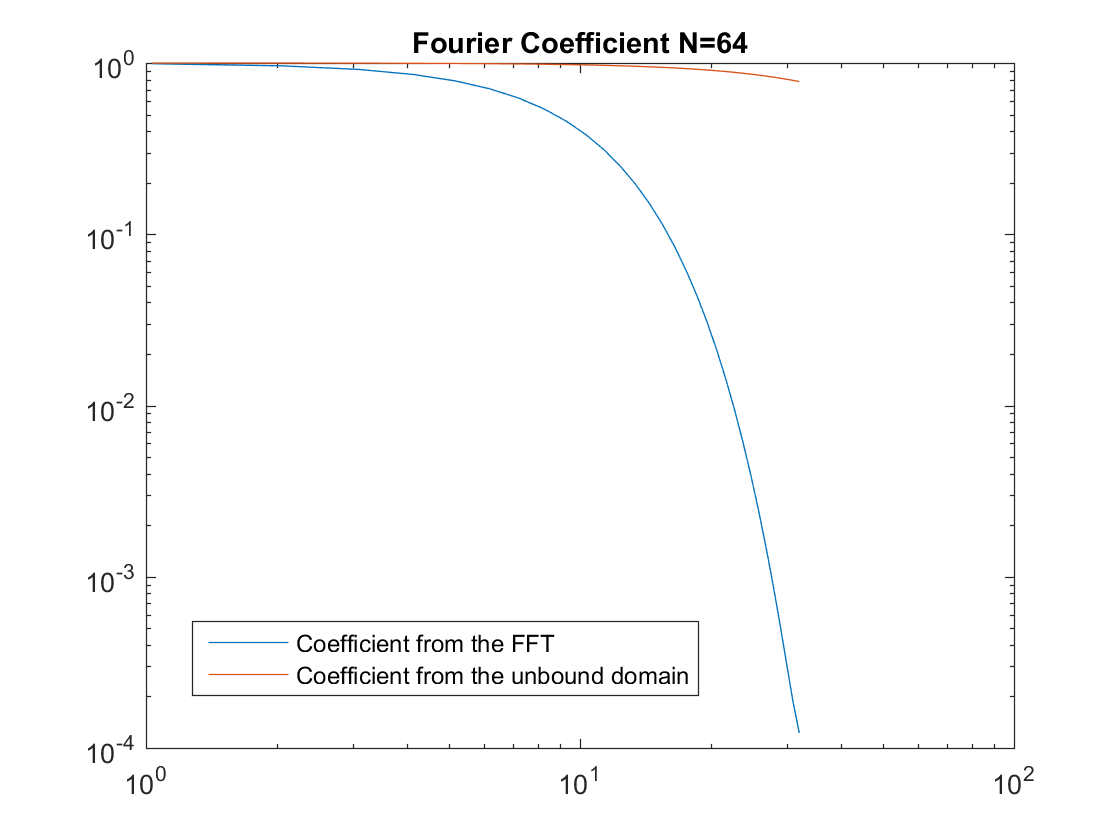
\includegraphics[scale=0.175]{img/fig0a.png}}
    \subfloat[N = 128]{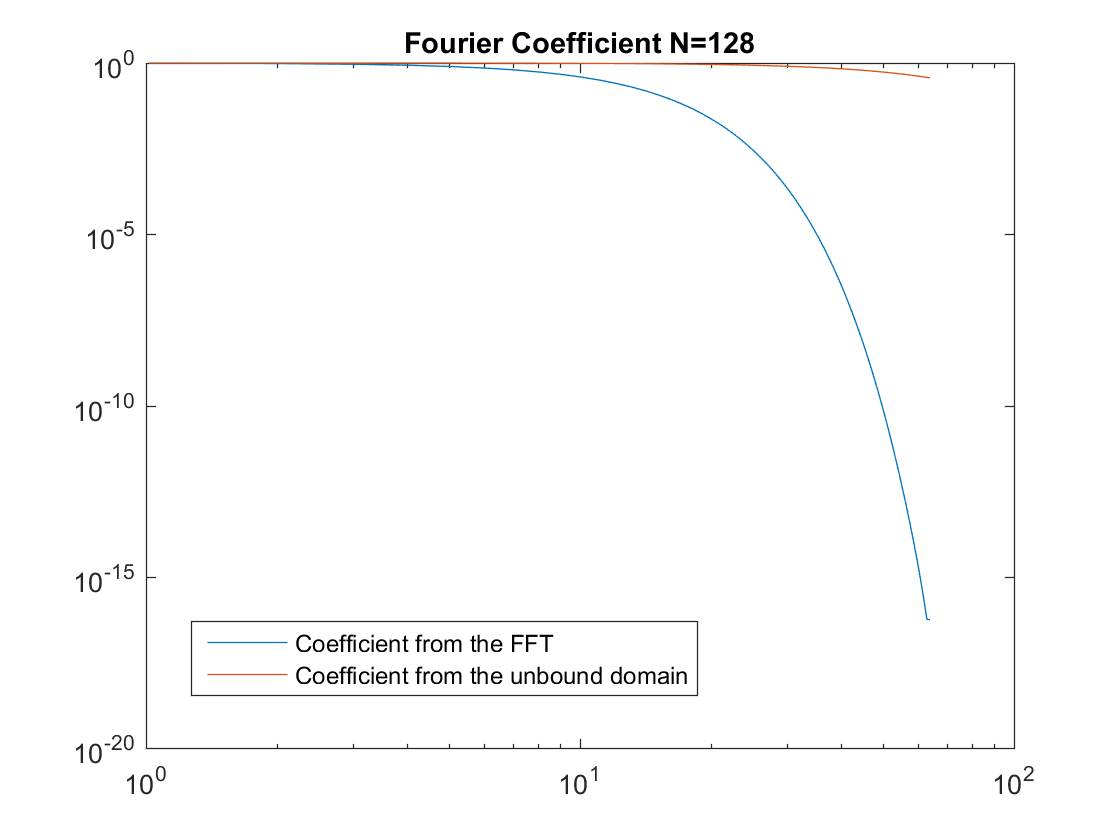
\includegraphics[scale=0.175]{img/fig0b.png}}
    \subfloat[N = 256]{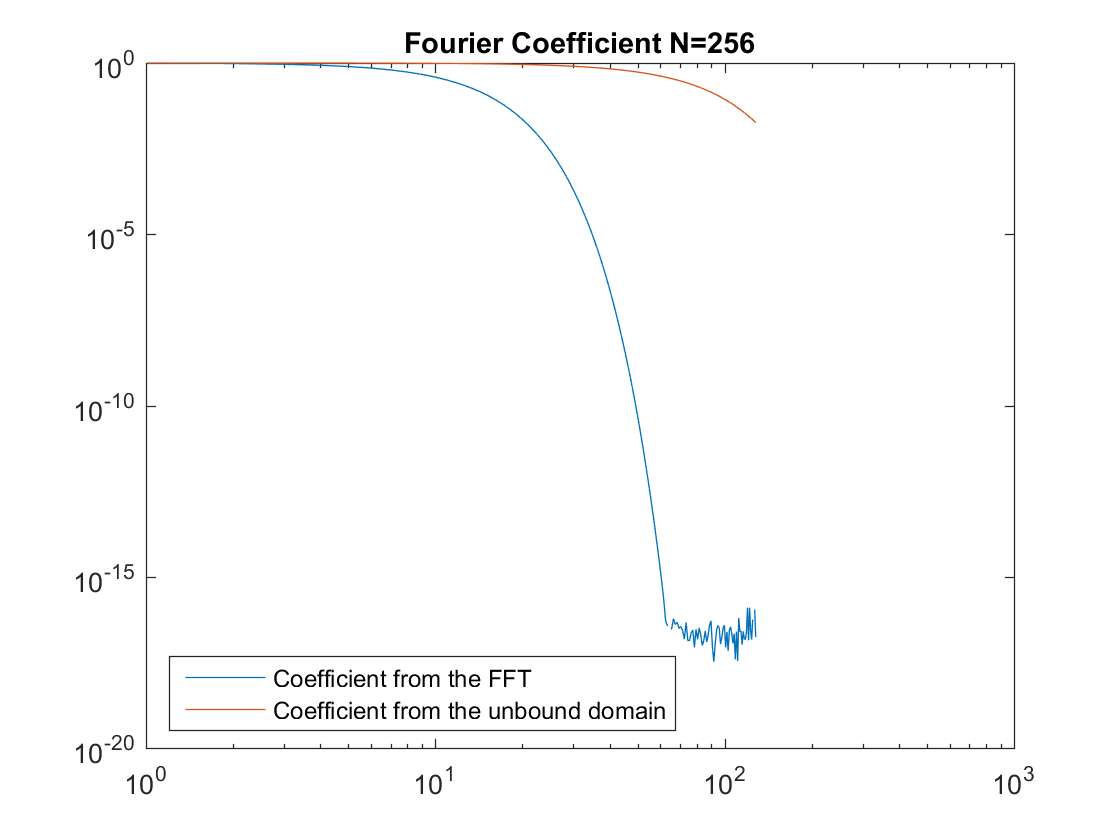
\includegraphics[scale=0.175]{img/fig0c.png}}
    \caption{Comparaison entre la séries de Fourier \\ et des coefficients de Fourier pour un N = 64,128 et 256}
    \label{fig0}
\end{figure}
\textit{Toutefois, au vue des graphs dans la figure \ref{fig0}, il semblerait que je n'ai pas effectué correctement ce qui était demander. Je possède encore quelques lacunes dans cette matière.} 

\newpage
\section{Centered and Partially Decentered Scheme}
Afin de construire notre méthode numérique pour résoudre les équations de convection-diffusions, nous utiliserons les différences finies. Ainsi, dans le cas de la convection, nous connaissons les schémas centrés classique d'ordre 2, et 4, définit respectivement ci-dessous.
\begin{equation}
    \begin{aligned}
        \frac{\partial u }{\partial x} & = \frac{U_{i+1} - U_{i-1}}{2h}\\
        \frac{\partial u }{\partial x} & = \frac{-U_{i+2}+8U_{i+1}-8U_{i-1}+U_{i+1}}{12h}\\
    \end{aligned}
\end{equation}
\\
Toutefois, nous nous intéresserons à un modèle décentré qui ne requiert que $U_{i-2}$, $U_{i-1}$, $U_{i}$, et $U_{i+1}$. Nous allons donc dérivée ce schéma à l'aide des polynômes de Taylor. Ainsi, nous retrouvons les polynômes suivants:\\
\begin{equation}
    \begin{aligned}
        U_{i+1} & = U_i +  \frac{\partial u }{\partial x} h +  \frac{\partial^2 u }{\partial x^2} \frac{h^2}{2} + \frac{\partial^3 u }{\partial x^3} \frac{h^3}{6} + \frac{\partial^4 u }{\partial x^4} \frac{h^4}{24} + ... \\ 
        U_{i-1} & = U_i -  \frac{\partial u }{\partial x} h +  \frac{\partial^2 u }{\partial x^2} \frac{h^2}{2} - \frac{\partial^3 u }{\partial x^3} \frac{h^3}{6} + \frac{\partial^4 u }{\partial x^4} \frac{h^4}{24} + ... \\
        U_{i-2} & = U_i - 2 \frac{\partial u }{\partial x} h + 4 \frac{\partial^2 u }{\partial x^2} \frac{h^2}{2} - 8 \frac{\partial^3 u }{\partial x^3} \frac{h^3}{6} + 16 \frac{\partial^4 u }{\partial x^4} \frac{h^4}{24} + ... \\ 
    \end{aligned}
\end{equation}
\\
De ce fait, nous retrouvons donc un systèmes d'équations représenté ci-dessous:\\
\begin{equation}
\begin{aligned}
        &= \alpha ( U_{i+1} - U_i ) +   \beta ( U_{i-1} - U_i ) +  \gamma ( U_{i-2} - U_i )   \\
        &= (\alpha-\beta-2\gamma) \frac{\partial u }{\partial x} h + (\alpha+\beta+4\gamma) \frac{\partial^2 u }{\partial x^2} \frac{h^2}{2} +  (\alpha-\beta-8\gamma)  \frac{\partial^3 u }{\partial x^3} \frac{h^3}{6} + \mathcal{O}(h^4)\\
\end{aligned}
\end{equation}
\\
Ainsi, en éliminant les autres termes que $\frac{\partial u }{\partial x}$, nous obtenons un schéma décentrée suivant:\\
\begin{equation}
    \frac{\partial u }{\partial x} = \frac{ U_{i-2} - 6U_{i-1} + 3U_{i} + 2U_{i+1}  }{6h} + \mathcal{O}(h^4)
\end{equation}
Ainsi, le schéma obtenu est d'ordre $\mathcal{O}(h^3)$, avec une error de troncation de $\mathcal{O}(h^4)$ comme nous pouvons le voir à travers le raisonnement. Nous étudierons maintenant la stabilité de ce schéma, pour se faire pour faisons une analyse modale. Pour $u_i(t) = \sum_j \widehat{U}_j (t) e^{ik_j x_i}$, nous obtenons les relations suivantes en utilisant le schéma décentré que nous avons trouvé :\\
\begin{equation}
    \begin{aligned}
    \frac{\partial u }{\partial x} & = \frac{ \widehat{U}_j (t) e^{ik_j x_{i-2}} - 6\widehat{U}_j (t) e^{ik_j x_{i-1}} + 3\widehat{U}_j (t) e^{ik_j x_{i}} + 2\widehat{U}_j (t) e^{ik_j x_{i+1}}  }{6h} \\
                                   & = \widehat{U}_j (t) \frac{ e^{ik_j x_{i-2}} - 6 e^{ik_j x_{i-1}} + 3 e^{ik_j x_{i}} + 2 e^{ik_j x_{i+1}}  }{6h} \\
                                   & =  \widehat{U}_j (t) \frac{ e^{-2ik_j h} - 6 e^{-ik_j h} + 3 + 2 e^{ik_j h}  }{6h}  e^{ik_j x_{i}} \\
    \end{aligned}
\end{equation}
Ainsi, en sachant que $\frac{\partial u }{\partial t} = \frac{ \partial \widehat{U} }{ \partial t } e^{ik_j x_{i}}$, dès lors nous avons les relations suivantes:
\begin{equation}
    \begin{aligned}
         \frac{ \partial \widehat{U} }{ \partial t } e^{ik_j x_{i}} & =  (-c)\widehat{U}_j (t) \frac{ e^{-2ik_j h} - 6 e^{-ik_j h} + 3 + 2 e^{ik_j h}  }{6h}  e^{ik_j x_{i}}\\
          \frac{ \partial \widehat{U} }{ \partial t } & =  (-c)\widehat{U}_j (t) \frac{ e^{-2ik_j h} - 6 e^{-ik_j h} + 3 + 2 e^{ik_j h}  }{6h}\\
          \lambda & =  (-c)\frac{ e^{-2ik_j h} - 6 e^{-ik_j h} + 3 + 2 e^{ik_j h}  }{6h}\\
    \end{aligned}
\end{equation}
En sachant qu'en pure convection, nous avons $ \frac{\partial u}{\partial t} = \lambda \widehat{U}$ pour le cas exact, nous pouvons maintenant, grâce aux résultats obtenu analyser les erreurs de phases et d'amplitude. Pour obtenir le graphe des erreurs d'amplitudes, nous calculons le module des $\lambda_k$ de chaque méthodes.
\begin{figure}[H]
    \centering
    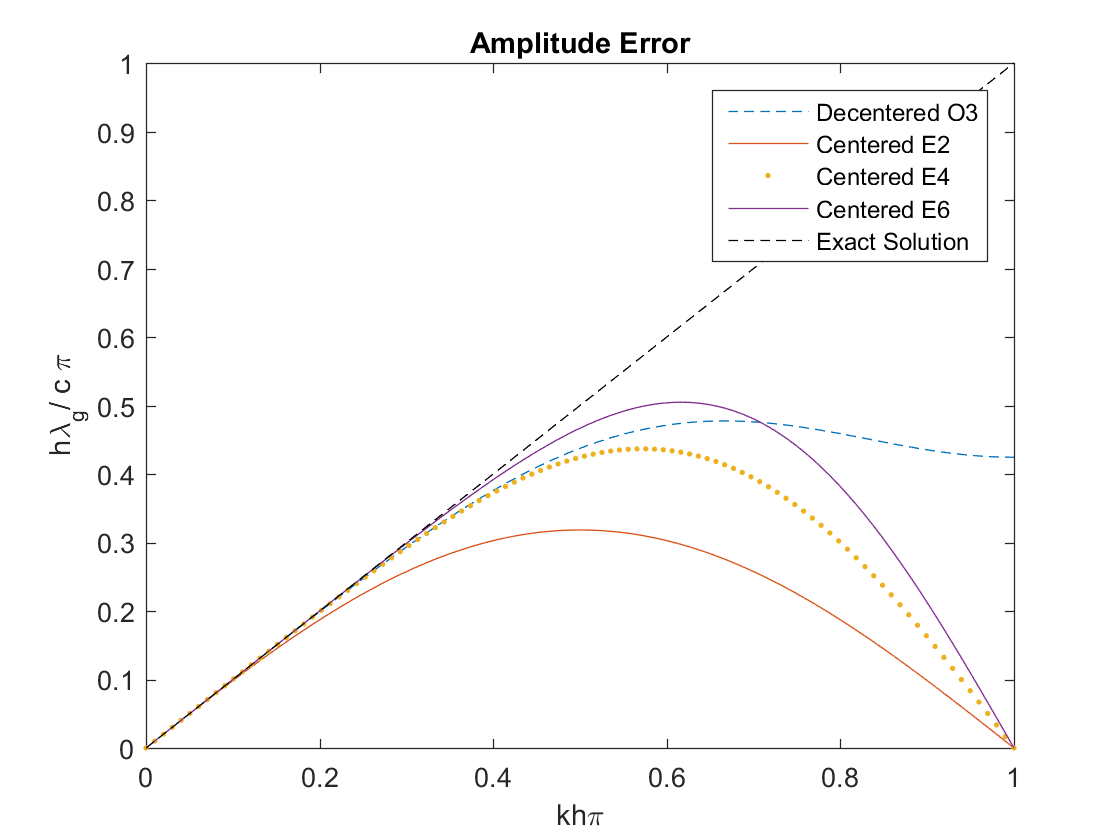
\includegraphics[scale=0.55]{img/fig1.png}
    \caption{Erreur d'amplitude des schémas decentrée d'ordre 3, E2,E4 et E6}
    \label{fig1}
\end{figure}
Ainsi, à l'aide de la figure \ref{fig1} sur l'erreur d'amplitude, nous observons aussi que ceux-ci auront tendance à diminuer petit à petit, pour le schéma décentré d'ordre 3, à partir de $\frac{kh}{\pi}  = 0.30$, vis à vis de la solution exacte, pour ensuite se stabilité dans les alentours de $\frac{kh}{\pi}  = 0.67$. Les autres schémas, E2, E4 et E6, ont par contre la tendance à diminuer très fortement jusqu'à s'annuler si bien que, pour ces schémas classiques, on aura des valeurs complètement erroné pour les grandes vitesses ce qui peut être désastreux pour la simulation même si le schéma d'ordre 6 fidèle plus longtemps à la solution exact. Le schéma décentré, qui possède une sorte de plateau, semble bien plus stable puisque les grands nombres d'ondes vont juste s'arrêter à un certain point tel qu'il donne l'impression qu'on fait une sorte de "cut-off" dans les nombres d'onde. Nous notons aussi que la précision du schéma E2 est vraiment faible puisqu'il s'écarte déjà de la solution exacte dès 0.15. \\
\\
Nous poursuivons maintenant notre chemin avec une analyse de stabilité, en regardant le comportement de ces derniers fonctions sur le plan complexe, présenté à la figure \ref{fig2}. Comme nous le doutions déjà, la zone de stabilité des schémas centrés est une droite confondant avec l'axe imaginaire. Dépendant du schéma centré, ils ne vont que s'allonger sur cette droite. Le schéma décentrée possède par contre une partie réelle, donnant lieux à tout une surface de stabilité. Ainsi, nous voyons bien que les schémas centrées sont instable, tandis que notre modèle décentrée est conditionnellement stable bien que ce dernier possède une diffusion numérique importante.  \\
\begin{figure}[H]
    \centering
    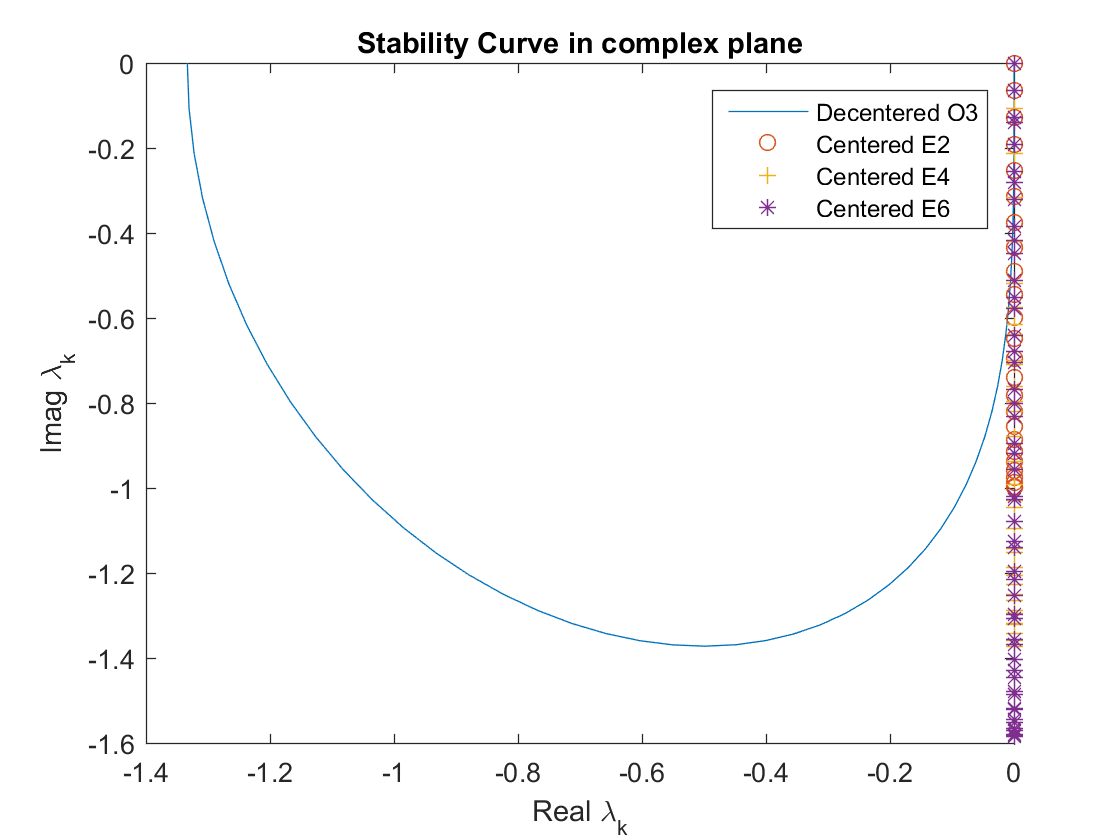
\includegraphics[scale=0.5]{img/fig2.png}
    \caption{Courbe de stabilité dans le plan complexe pour $0 < \frac{kh}{\pi} < 1$}
    \label{fig2}
\end{figure}

\newpage
\section{Simulation de la convection}
\subsection{Taille des meshes}
Ainsi, nous allons pouvoir concevoir notre simulation numérique des effets de convection et de diffusion. Pour ce faire, nous utiliserons, pour chacun des schémas de différence finies, l'intégrateur numérique Runge-Kutta 4 (RK4). Dans un premier temps,si bien que nous allons plus nous intéressé à la partie convective, nous fixons ainsi temporairement $\nu = 0$. Pour nous aider dans la confection de cette simulation, nous nous aiderons des relations adimensionnels suivant: $\frac{h}{\sigma}$,le rapport entre la taille de la "mesh" sur $\sigma$, N, le nombre d'éléments discrétisé, obtenu par $N = \frac{L}{h}$, CFL, pour $CFL = \frac{c\Delta t}{h}$, la condition de Courant–Friedrichs–Lewy, $\frac{ct}{L}$, le temps adimensionalisé, \textbf{qui, par facilité de notation, sera appelé dans ce rapport par $\tau$}. Enfin, nous fixons notre $\sigma$ à $\frac{L}{32}$ un domaine assez large pour qu'on puisse définir un domaine numérique périodique, de même que notre CFL sera de 1.\\

Nous utiliserons 5 schémas de différence finie différents que nous comparerons chacun par rapport aux uns et aux autres, mais aussi à la solution exacte analytique: la Décentré d'ordre 3, Euler Explicite Centré 2 (E2), Euler Explicite Centré 4 (E4), Euleur Implicite 4 (I4), et Euleur Implicite 6 (I6). En ce qui concerne les schémas implicites, nous utiliserons l'algorithme de Thomas pour résoudre le système tridimensionnel qui nous garantis une complexité temporelle de $\mathcal{O}(n)$. Dans un premier temps, nous allons nous intéresser à l'influence de h dans notre simulation numérique. De ce fait, nous allons observé le comportement de chacun des schémas pour $\frac{h}{\sigma} = \frac{1}{2}, \frac{1}{4}$, et $\frac{1}{8}$ correspondant au nombre de point N = 64, 128, et 256. Afin de mieux visualisé les éléments, les graphes seront en fonction de n, le n-nième éléments du domaine discrétisé, puisque nous travaillons dans une "box" de taille L, contenant N éléments. Afin de facilité la lecture, nous adimentionaliserons U par $U' = \frac{\sqrt{\pi \sigma^2}}{Q} U$.\\

Comme nous le voyons sur les figures \ref{fig3a}, \ref{fig3b}, et \ref{fig3c}, la représentation des points pour $\tau 0.25$, nous observons une nette amélioration entre 64 points et 256 points. De faite, pour 64 points, figure  \ref{fig3a}, tous nos schémas de différence finie s'écartent drastiquement de la solution exacte. Bien que les schémas implicites essayent de rester le plus fidèle possible, les schémas centrés ont explosé et commence à osciller sur la gauche de la courbe. De plus, le schéma décentré lui aussi éprouve des difficultés à se maintenir stable. La situation s'améliore dans le cas avec 128 points, figure  \ref{fig3b}, où seul E2 est instable. Toutefois, le schéma décentré ne nous donne toujours pas la bonne solution contrairement aux schémas implicites, et E4 qui tendent de plus en plus, bien que ce n'est pas encore parfaite comme nous pouvons voir sur le zoom-in, figure  \ref{fig3ba}. C'est avec 256 points, figure  \ref{fig3c}, que les schémas implicites, et E4, se confondent avec la solution exacte. Nous pouvons aussi remarquer que le schéma E2 possède encore des imprécisions, puisqu'il semble même avoir un retard par rapport à la solution exacte comme on peut le voir sur le zoom-in, figure  \ref{fig3ca}. Bien que son amplitude n'est pas exacte, le schéma décentré d'ordre 3 a ses points bien aligné avec ceux de la solution exacte et des autres schémas implicites. Toutefois, nous avons vu, un peu au dessus, que la solution décentré a une tendance à diffuser, ce qui semble apparaître ici. \\

\textit{Note: Le code en C, ci-joint, a été programmer pour être compatible avec un ordinateur fonctionnant sous linux (WSL Ubuntu 14.04), il se peut qu'il y aie des librairies qui manque lors de la compilation du code si on le fait sur un autre OS.}



\newpage
\begin{figure}[H]
    \centering
    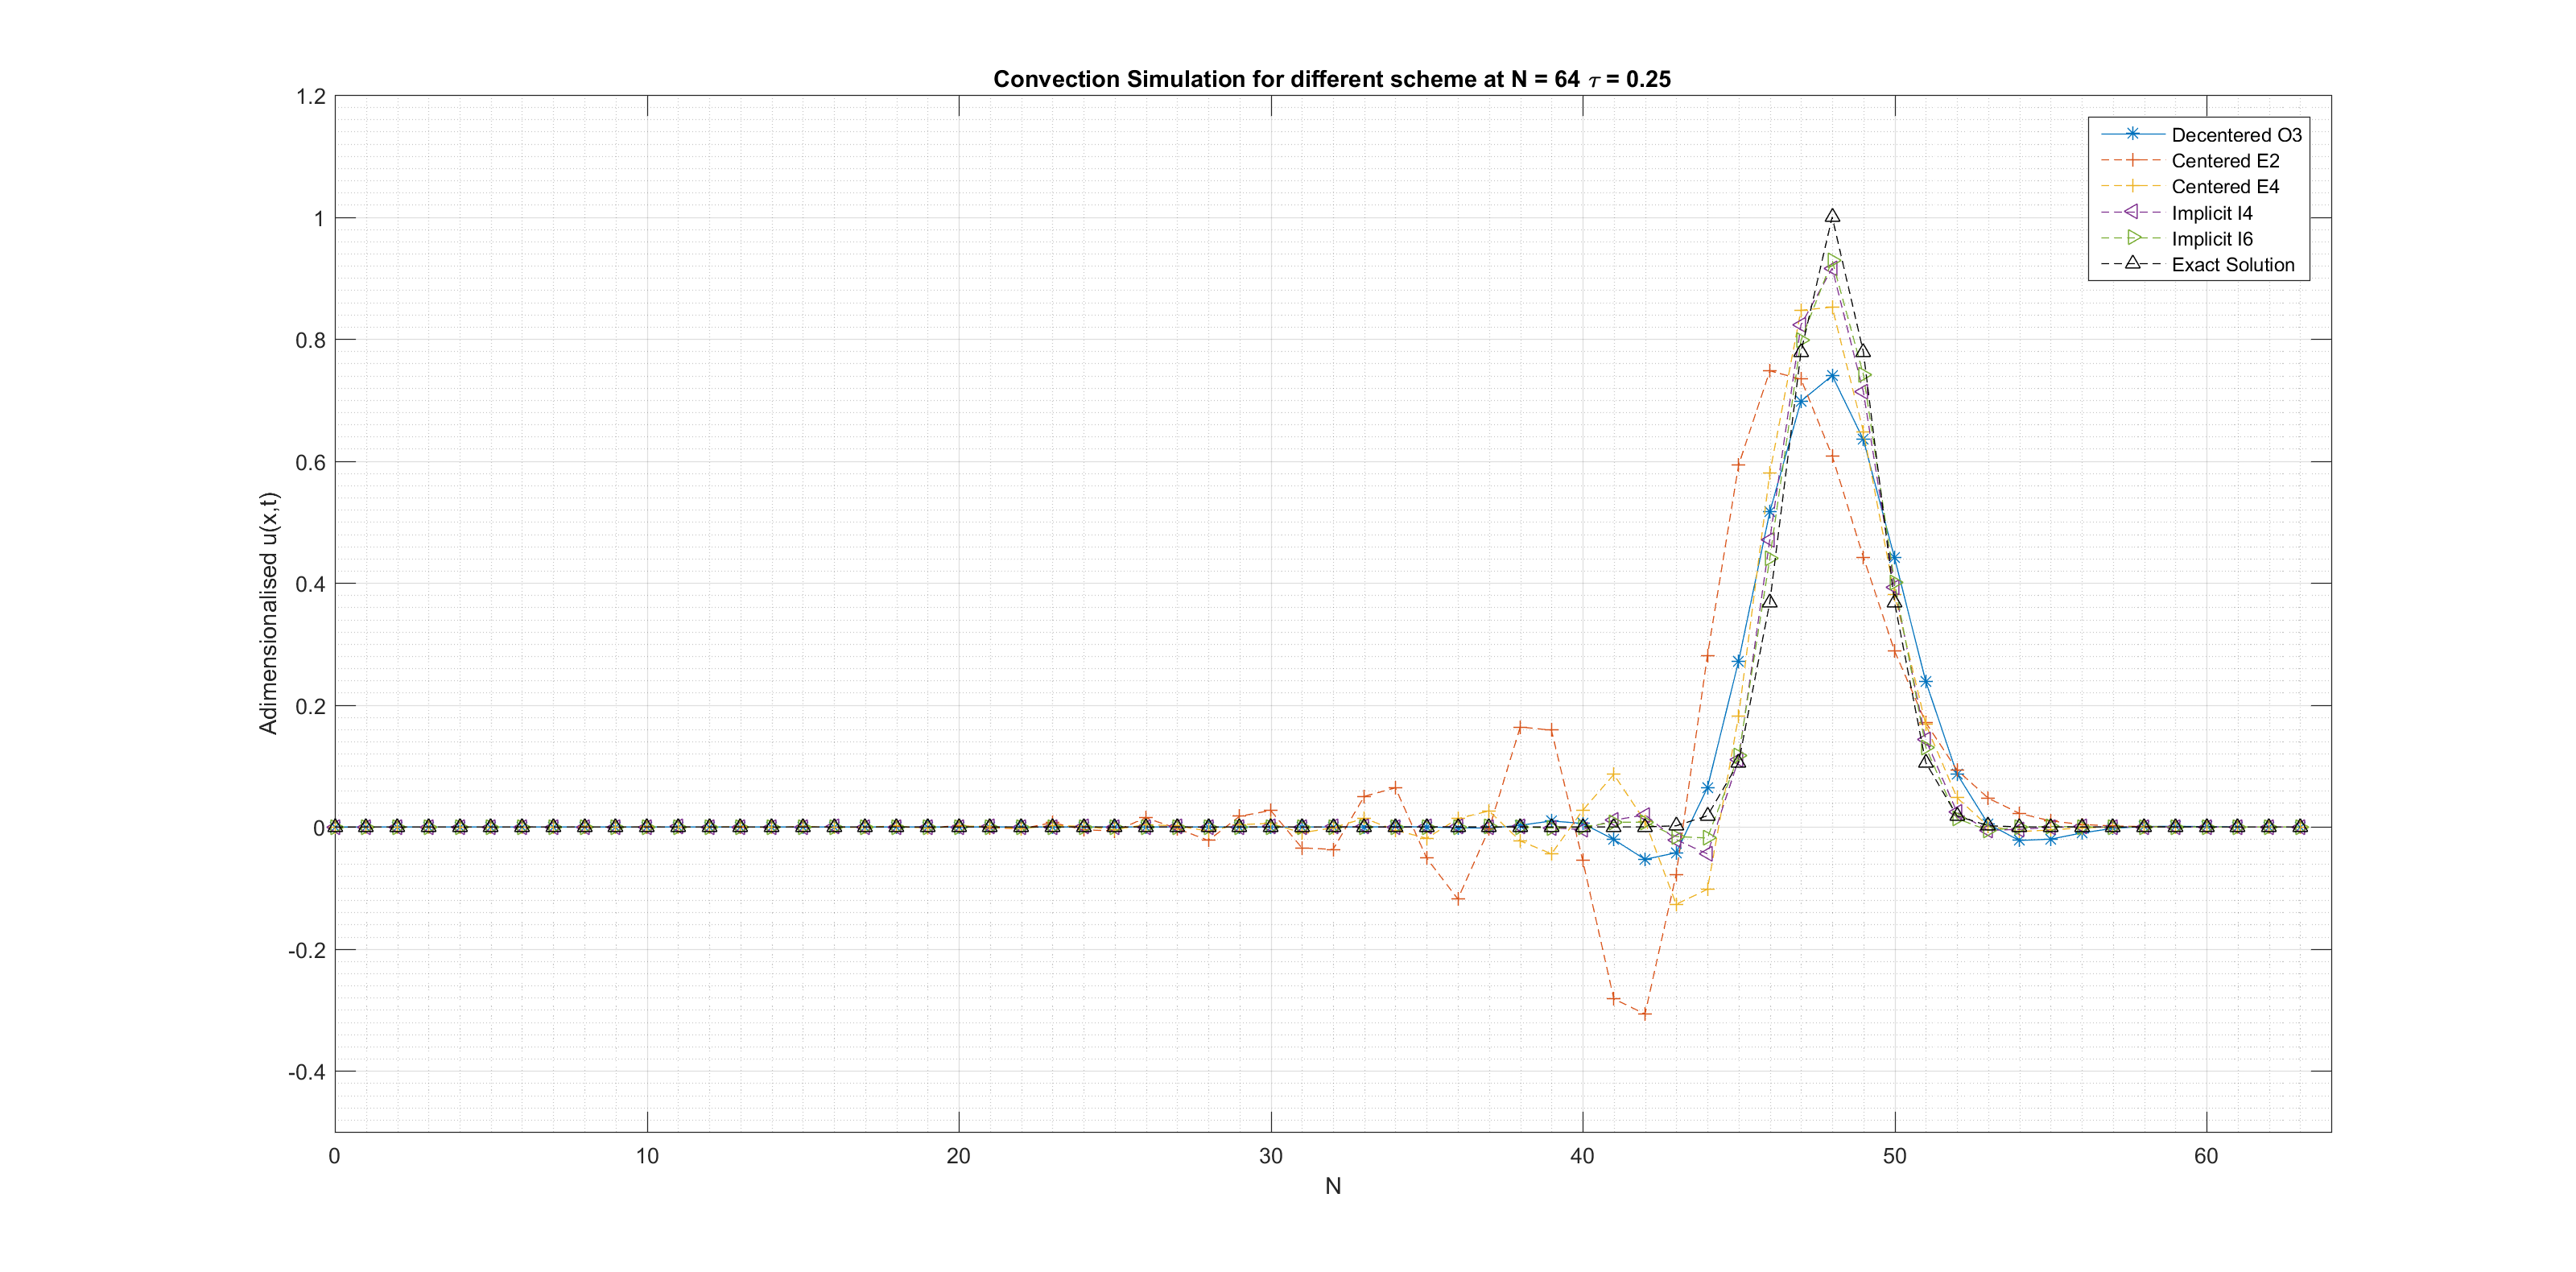
\includegraphics[scale=0.27,angle=90]{img/fig3a.png}
    \caption{Réprésentation de $\frac{\sqrt{\pi \sigma^2}}{Q} U$ à $\tau = 0.25$ N = 64}
    \label{fig3a}
\end{figure}
\begin{figure}[H]
    \centering
    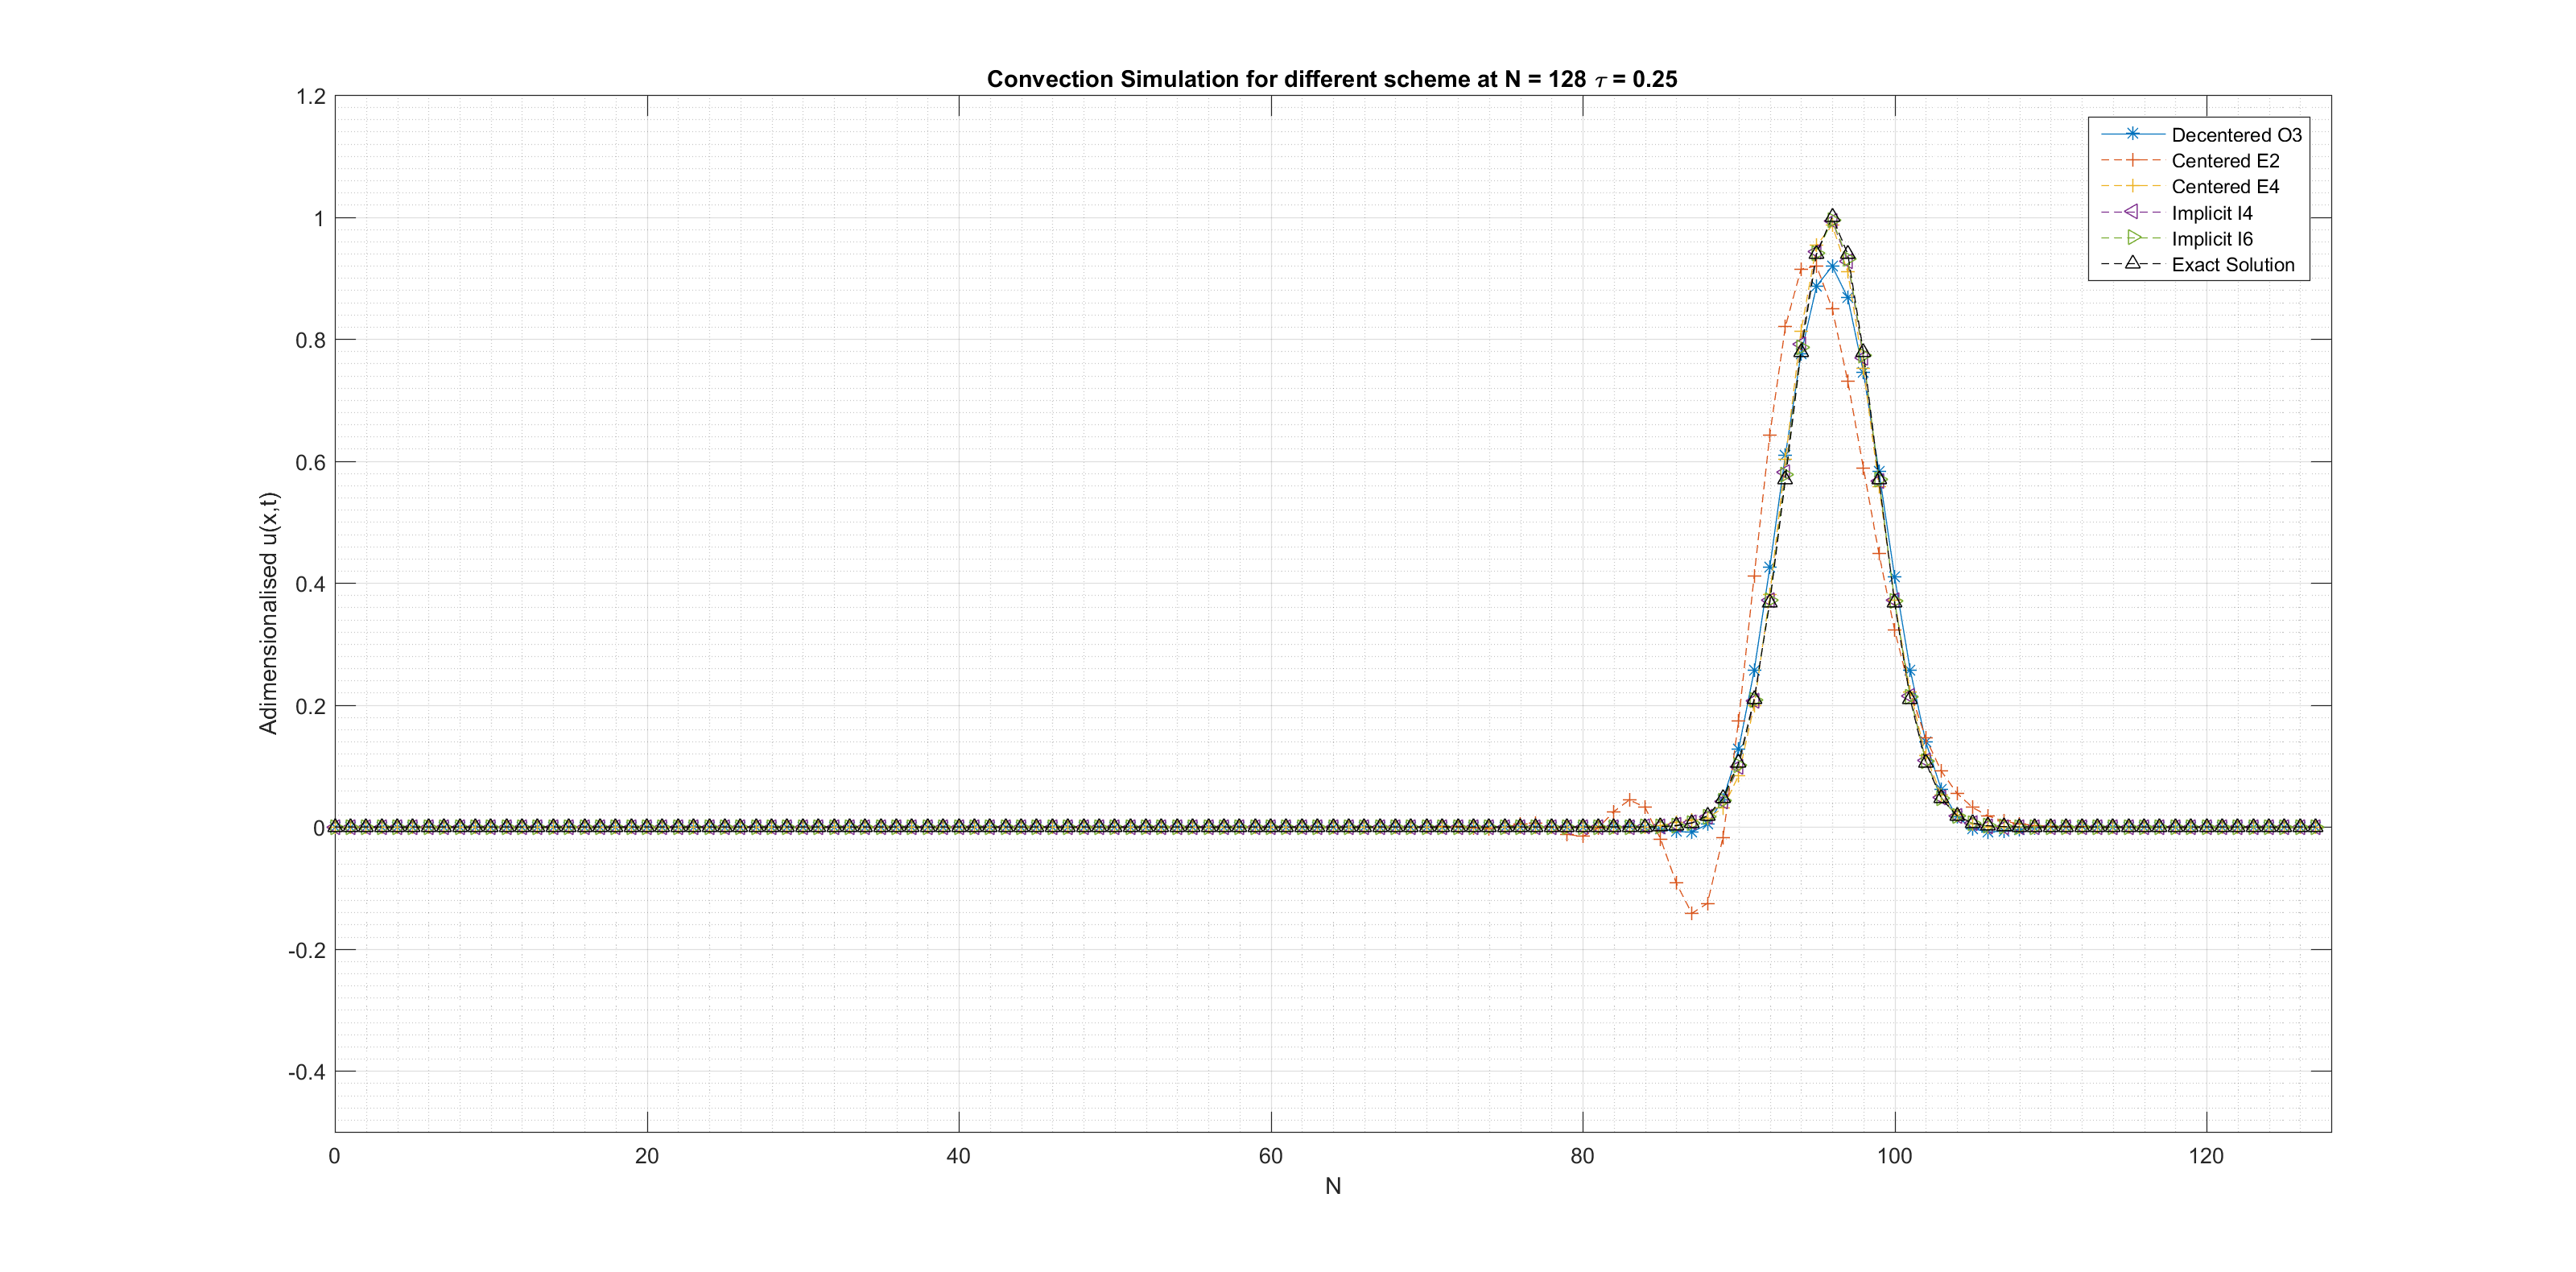
\includegraphics[scale=0.27,angle=90]{img/fig3b.png}
    \caption{Réprésentation de $\frac{\sqrt{\pi \sigma^2}}{Q} U$ à $\tau = 0.25$ N = 128}
    \label{fig3b}
\end{figure}
\begin{figure}[H]
    \centering
    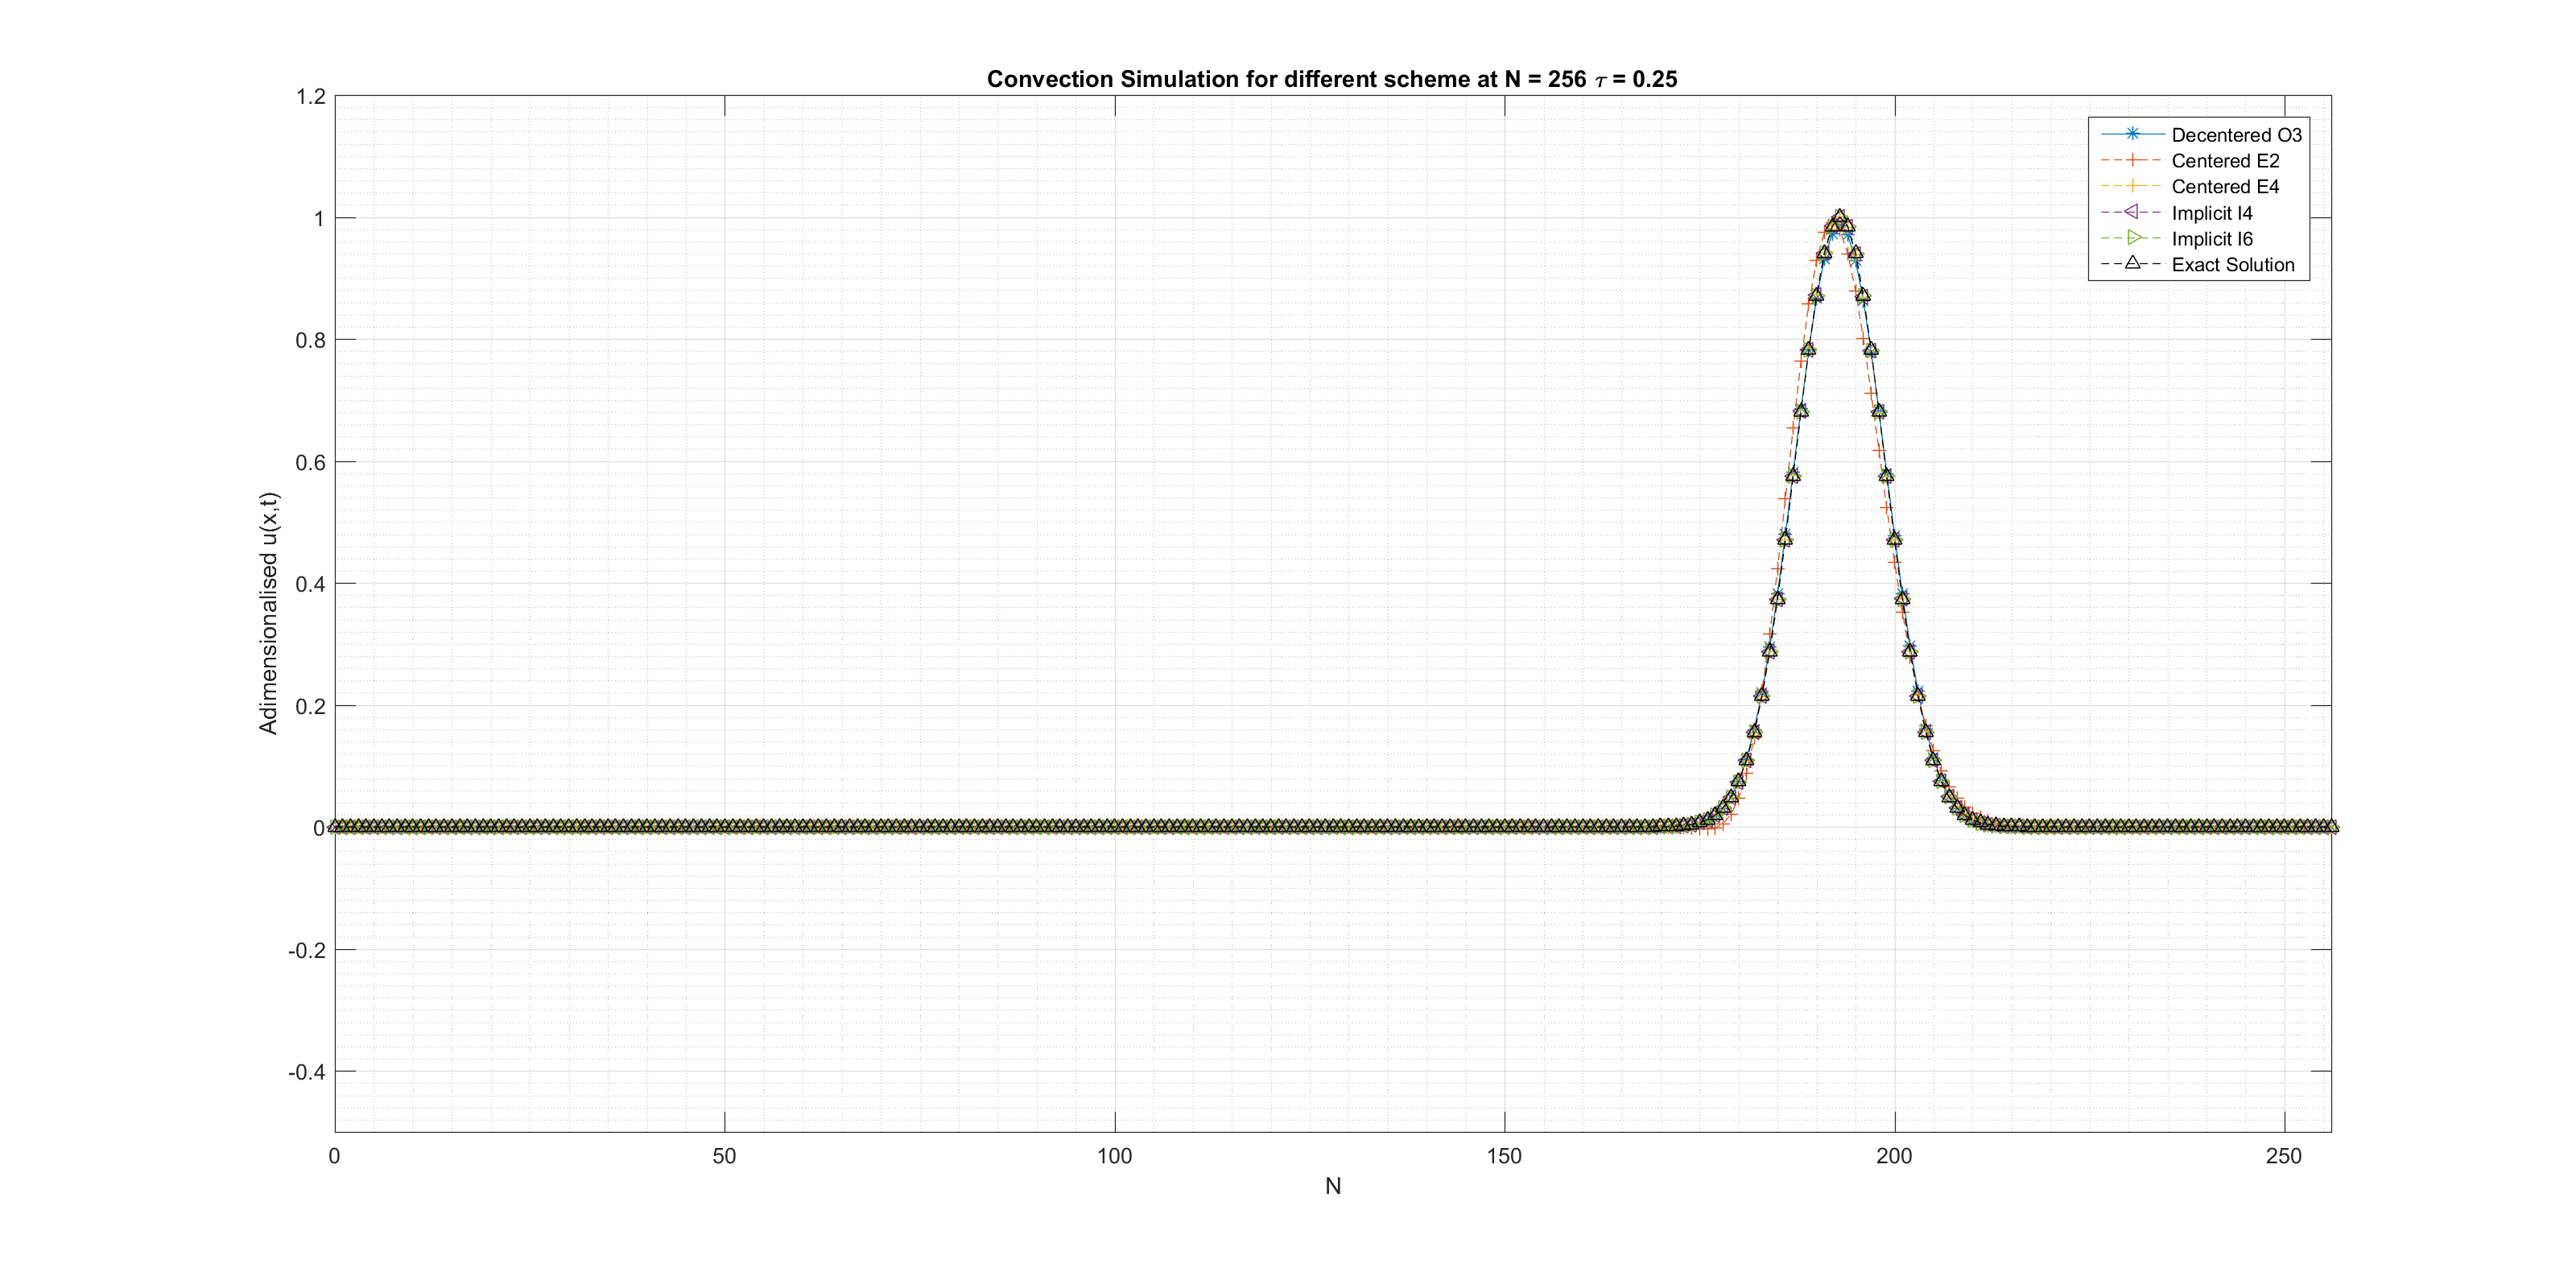
\includegraphics[scale=0.27,angle=90]{img/fig3c.png}
    \caption{Réprésentation de $\frac{\sqrt{\pi \sigma^2}}{Q} U$ à $\tau = 0.25$ N = 256}
    \label{fig3c}
\end{figure}
\begin{figure}[H]
    \centering
    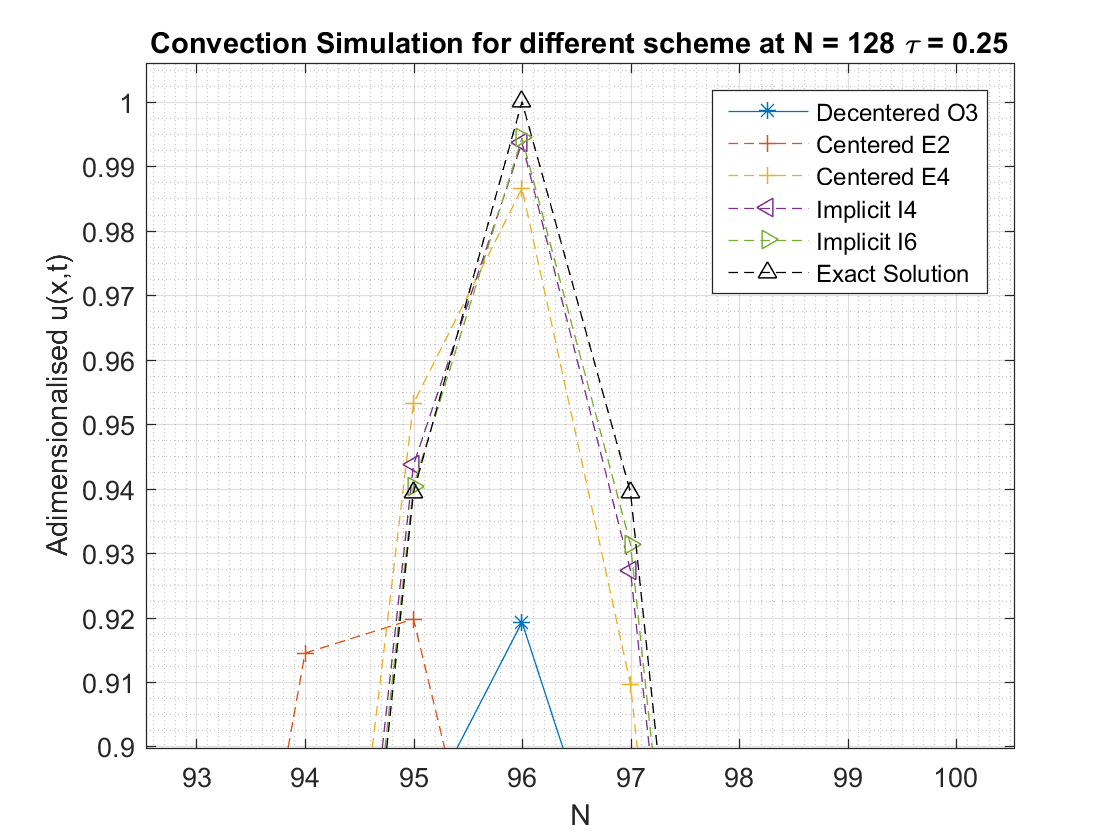
\includegraphics[scale=0.45]{img/fig3ba.png}
    \caption{Réprésentation de $\frac{\sqrt{\pi \sigma^2}}{Q} U$ à $\tau = 0.25$ N = 128 , zoom-in}
    \label{fig3ba}
\end{figure}
\begin{figure}[H]
    \centering
    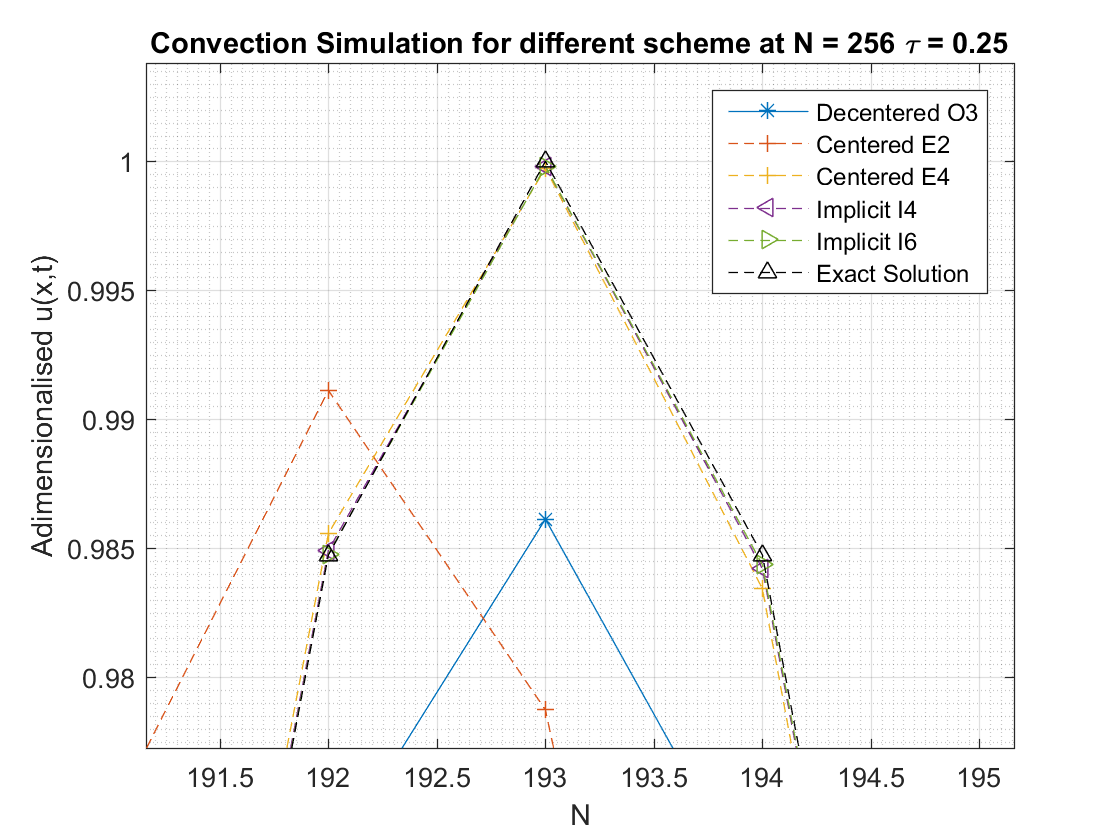
\includegraphics[scale=0.45]{img/fig3ca.png}
    \caption{Réprésentation de $\frac{\sqrt{\pi \sigma^2}}{Q} U$ à $\tau = 0.25$ N = 256 , zoom-in}
    \label{fig3ca}
\end{figure}


\newpage
\subsection{Convection à travers plusieurs temps}
Nous allons maintenant nous intéresser aux comportements de nos schémas sur quelques temps spécifiques. Pour se faire, nous utiliserons 256 points que nous simulerons pour $\frac{ct}{L} = \tau = $ 0.25, 0.50, 0.75, 1.00, ce qui correspond respectivement à un quart de période, demi période, trois-quart de période, et un période entier. Comme nous pouvons voir sur les figures  \ref{fig4a1}, \ref{fig4a2}, \ref{fig4b1}, \ref{fig4b2}, \ref{fig4c1}, \ref{fig4c2}, \ref{fig4d1}, alors que la E2 était à peu près stable \ref{fig4d2}, une instabilité apparaît dès qu'il travers la frontière, qui s'intensifie de plus en plus au cours du temps. Les autres schémas restent par contre stable malgré le passage à travers de la frontière du domaine, de même que les schémas implicites, et le schéma E4 restent toujours fidèles à la solution exacte. Enfin, le schéma décentré d'ordre possède une amplitude bien plus petite comme on l'avait déjà remarquer. \\

\textit{Note: Pour avoir une visibilité des schémas, les graphes on été séparer en deux: les schémas explicites centrés d'un coté, et les schéma implicites de l'autre, avec la solution exacte et le schéma décentré sur chacun des deux pour pouvoir mieux comparer.}


\begin{figure}[H]
    \centering
    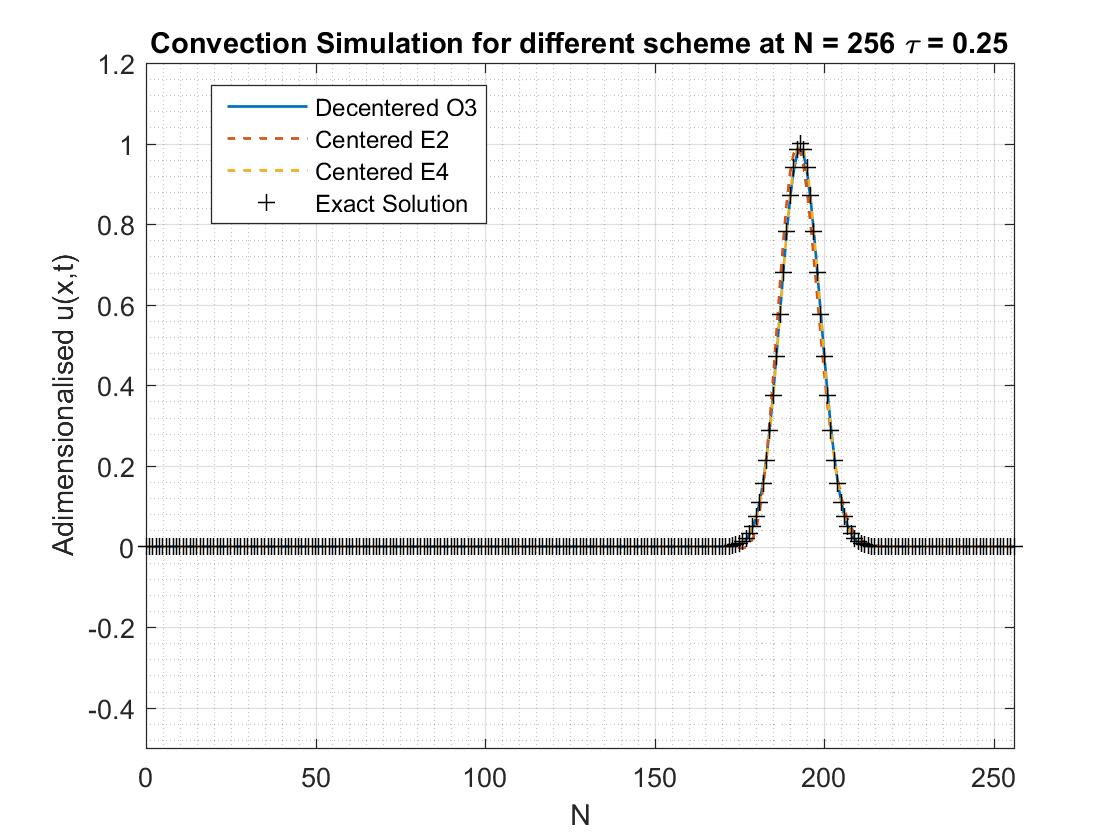
\includegraphics[scale=0.45]{img/fig4a1.png}
    \caption{Réprésentation de $\frac{\sqrt{\pi \sigma^2}}{Q} U$ à $\tau = 0.25$ N = 256 - Schéma Explicite}
    \label{fig4a1}
\end{figure}
\begin{figure}[H]
    \centering
    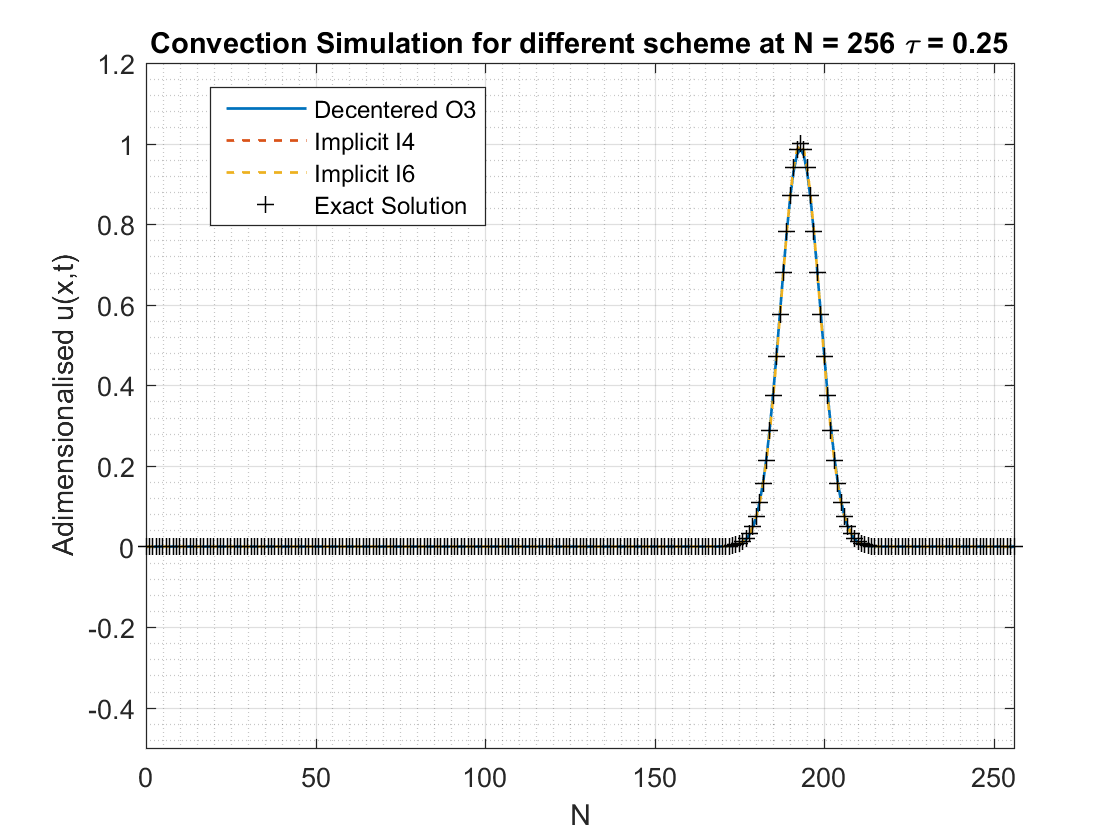
\includegraphics[scale=0.45]{img/fig4a2.png}
    \caption{Réprésentation de $\frac{\sqrt{\pi \sigma^2}}{Q} U$ à $\tau = 0.25$ N = 256 - Schéma Implicite}
    \label{fig4a2}
\end{figure}
\begin{figure}[H]
    \centering
    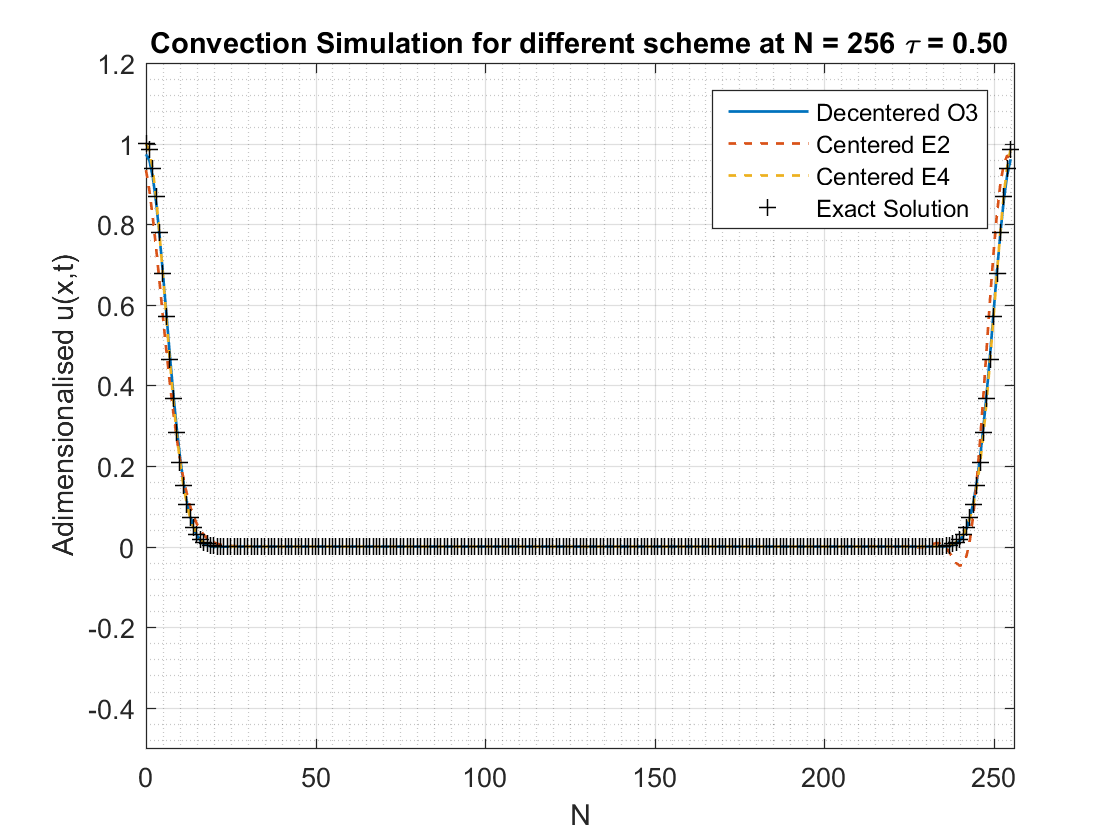
\includegraphics[scale=0.45]{img/fig4b1.png}
    \caption{Réprésentation de $\frac{\sqrt{\pi \sigma^2}}{Q} U$ à $\tau = 0.50$ N = 256 - Schéma Explicite}
    \label{fig4b1}
\end{figure}
\begin{figure}[H]
    \centering
    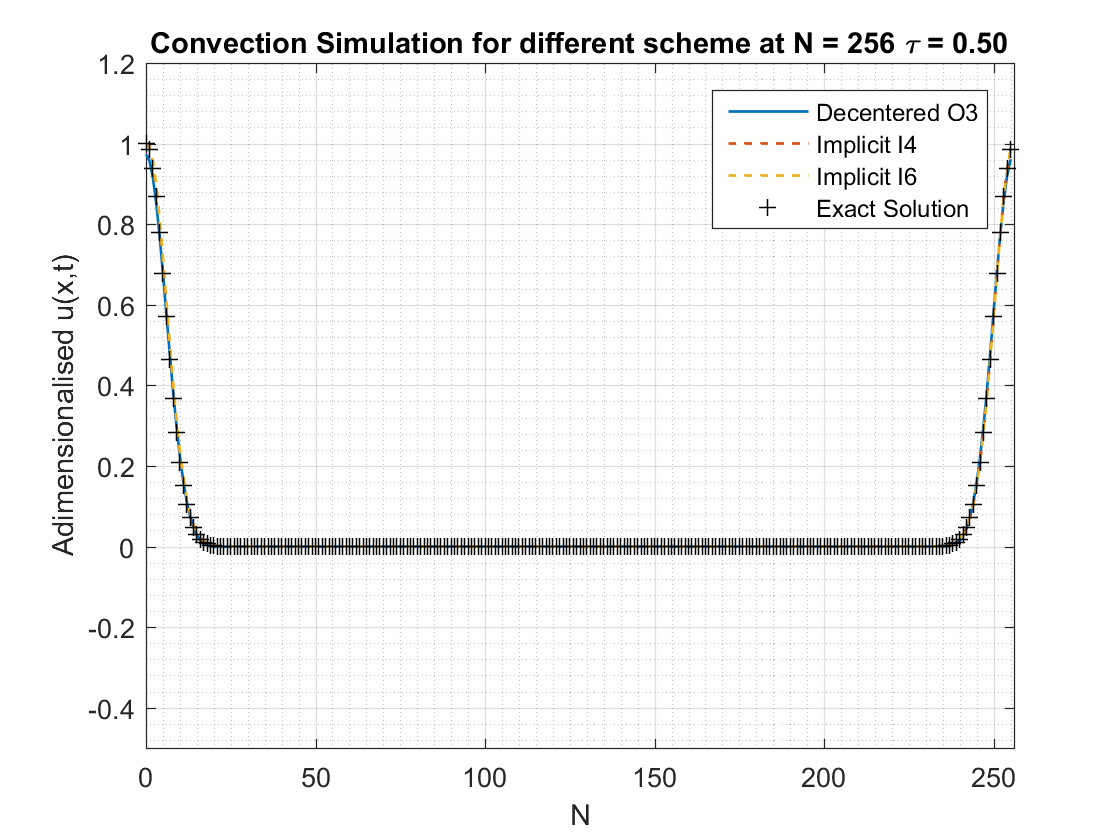
\includegraphics[scale=0.45]{img/fig4b2.png}
    \caption{Réprésentation de $\frac{\sqrt{\pi \sigma^2}}{Q} U$ à $\tau = 0.50$ N = 256 - Schéma Implicite}
    \label{fig4b2}
\end{figure}
\begin{figure}[H]
    \centering
    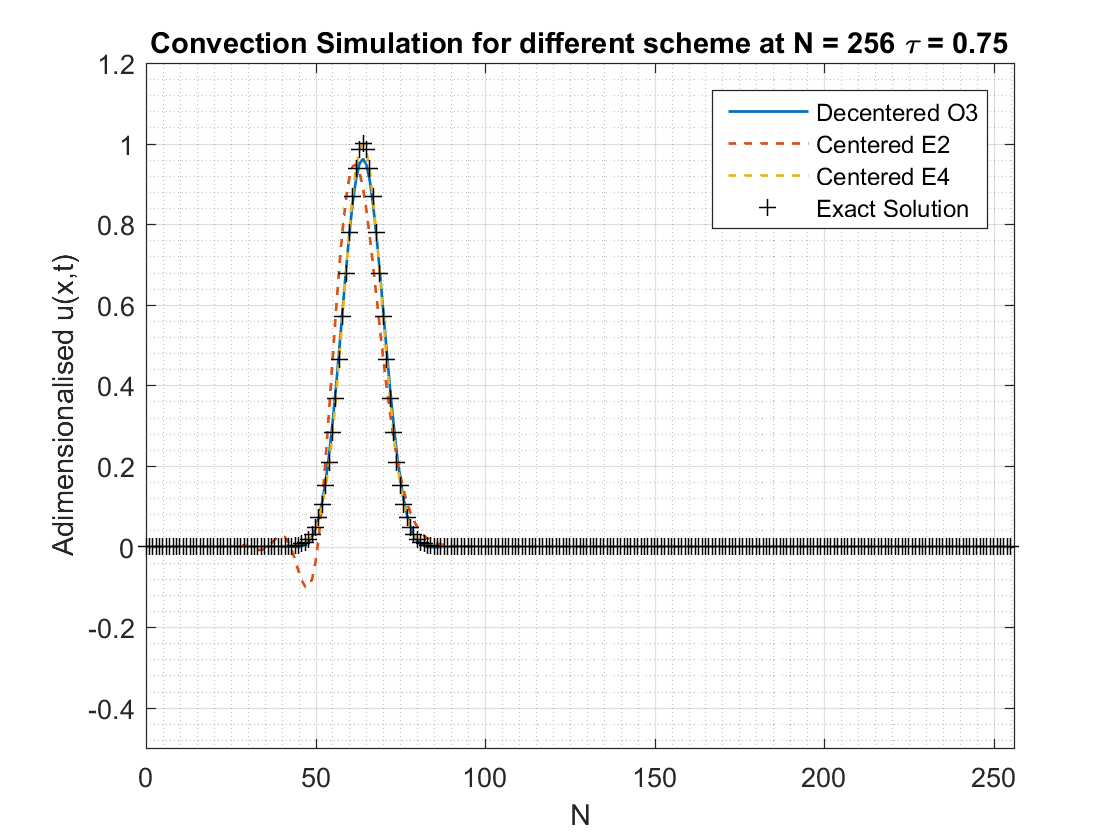
\includegraphics[scale=0.45]{img/fig4c1.png}
    \caption{Réprésentation de $\frac{\sqrt{\pi \sigma^2}}{Q} U$ à $\tau = 0.75$ N = 256 - Schéma Explicite}
    \label{fig4c1}
\end{figure}
\begin{figure}[H]
    \centering
    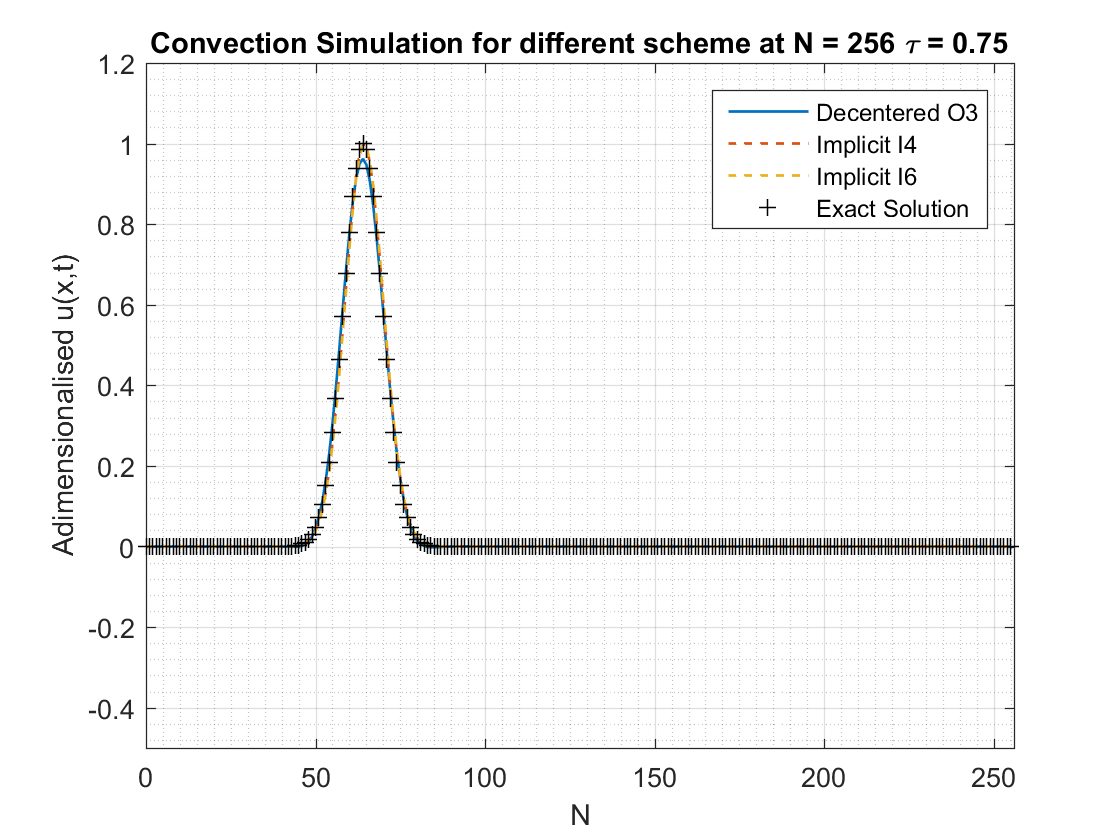
\includegraphics[scale=0.45]{img/fig4c2.png}
    \caption{Réprésentation de $\frac{\sqrt{\pi \sigma^2}}{Q} U$ à $\tau = 0.75$ N = 256 - Schéma Implicite}
    \label{fig4c2}
\end{figure}
\begin{figure}[H]
    \centering
    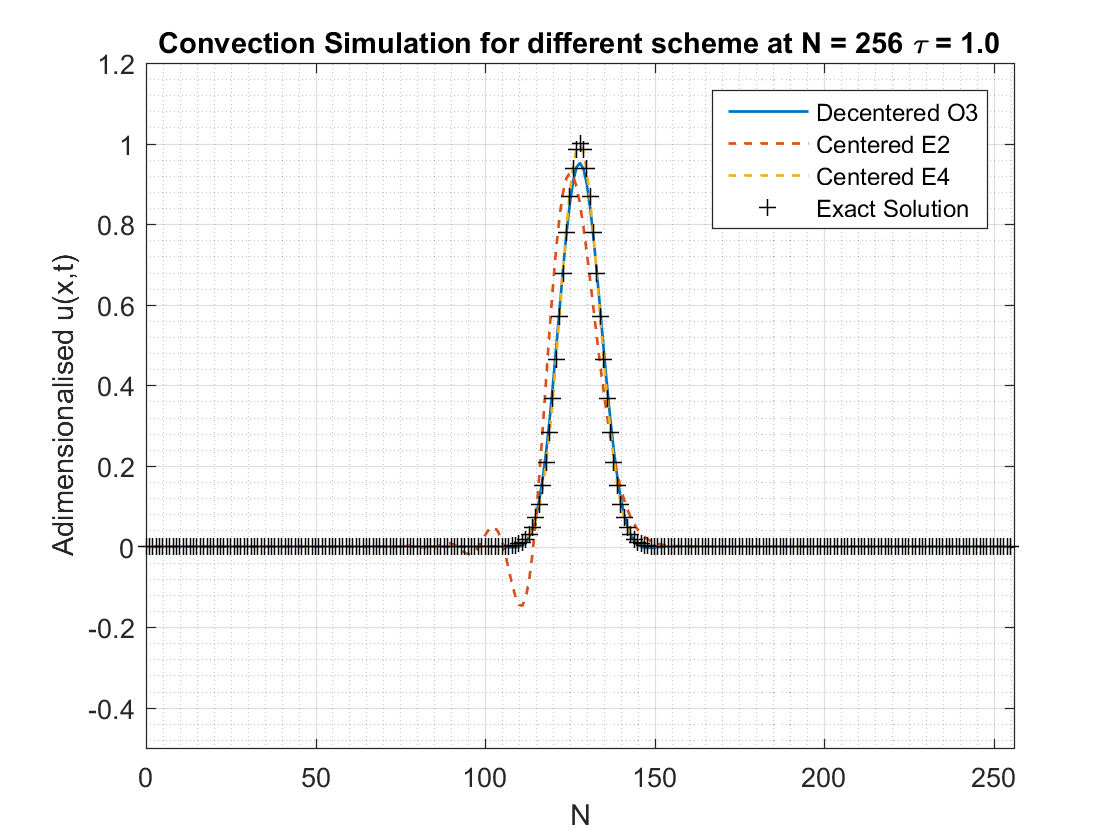
\includegraphics[scale=0.45]{img/fig4d1.png}
    \caption{Réprésentation de $\frac{\sqrt{\pi \sigma^2}}{Q} U$ à $\tau = 1.00$ N = 256 - Schéma Explicite}
    \label{fig4d1}
\end{figure}
\begin{figure}[H]
    \centering
    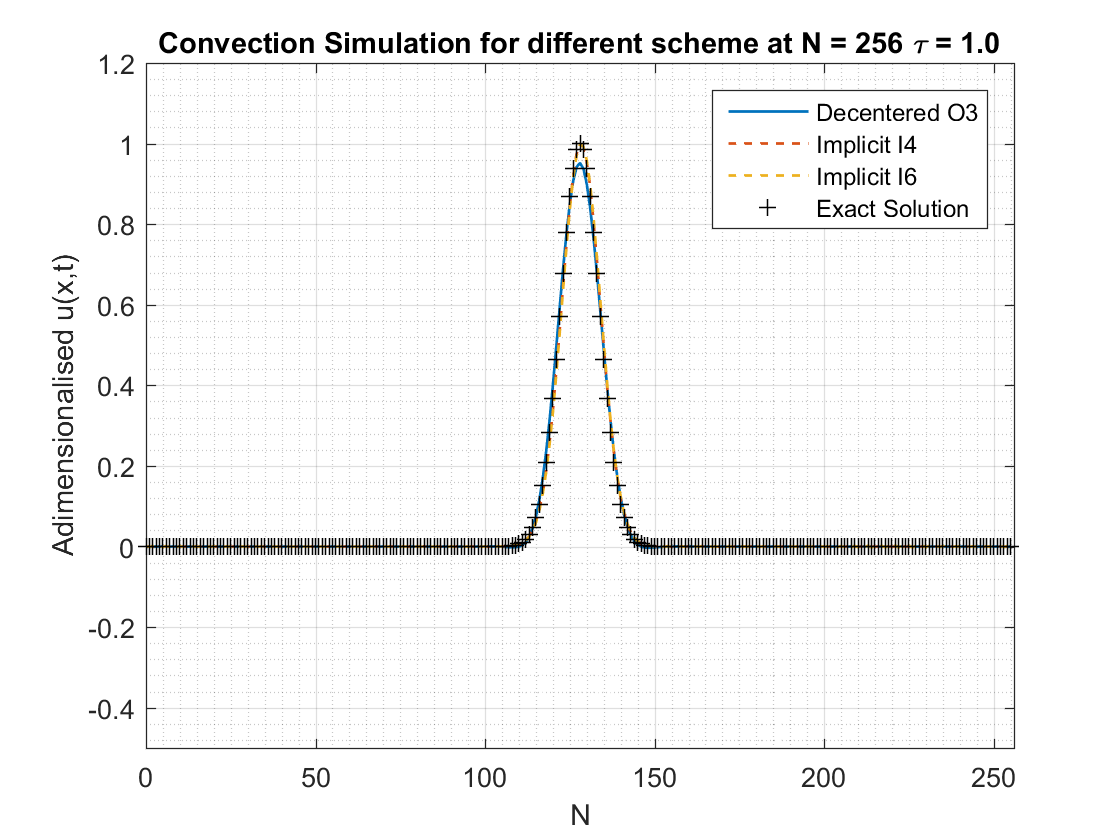
\includegraphics[scale=0.45]{img/fig4d2.png}
    \caption{Réprésentation de $\frac{\sqrt{\pi \sigma^2}}{Q} U$ à $\tau = 1.00$ N = 256 - Schéma Implicite}
    \label{fig4d2}
\end{figure}

Maintenant, nous analyserons en détails le comportement de nos schémas en appliquant de petit éléments de diagnostique définit comme suit:\\
\begin{equation}
    \begin{aligned}
        Q_h^n & = h {\sum}_i u_i^n \\
        E_h^n & = h {\sum}_i \frac{(u_i^n)^2}{2} \\
        R_h^n & = \sqrt{h {\sum}_i (u_i^n - u(x_i,t^n))^2}
    \end{aligned}
\end{equation}
Ces derniers sont donc calculé à chaque pas de temps, si bien que nous obtenons au final une évolution temporelle de ces éléments de diagnostique, réprésenté ci dessous par les figures  \ref{fig6a}, \ref{fig6b},et \ref{fig6c}. Nous remarquons dans un premier lieu que le Q reste constant pour chacun des schémas. Toutefois, ce n'est pas le cas pour $E_h^n$ où on remarque clairement que la méthode décentrée décroît alors que le reste sont constant. Ce qui confirme le fait que le schéma semble bel et bien décroître, et qu'il y a donc une diffusion numérique comme on l'avait annoncé avec les graphes d'erreur d'amplitude et de stabilité. En ce qui concerne de $R_h^n$, il nous montre bien que le schéma E2 dégénère complètement au fil du temps, de même que l'erreur fait par le schéma décentrée est relativement grand comparer aux restes des schémas. En utilisant la figure \ref{fig9}, on voit qu'on a un ordre de convergence d' $\mathcal{O}(10^{-1})$ pour E4 et la décentré d'ordre 3, et un ordre de convergence qui tourne autour de $\mathcal{O}(10^{-2})$ pour I4 et I6, et enfin la E2 aurait un ordre de $\mathcal{O}(1)$.

\begin{figure}[H]
    \centering
    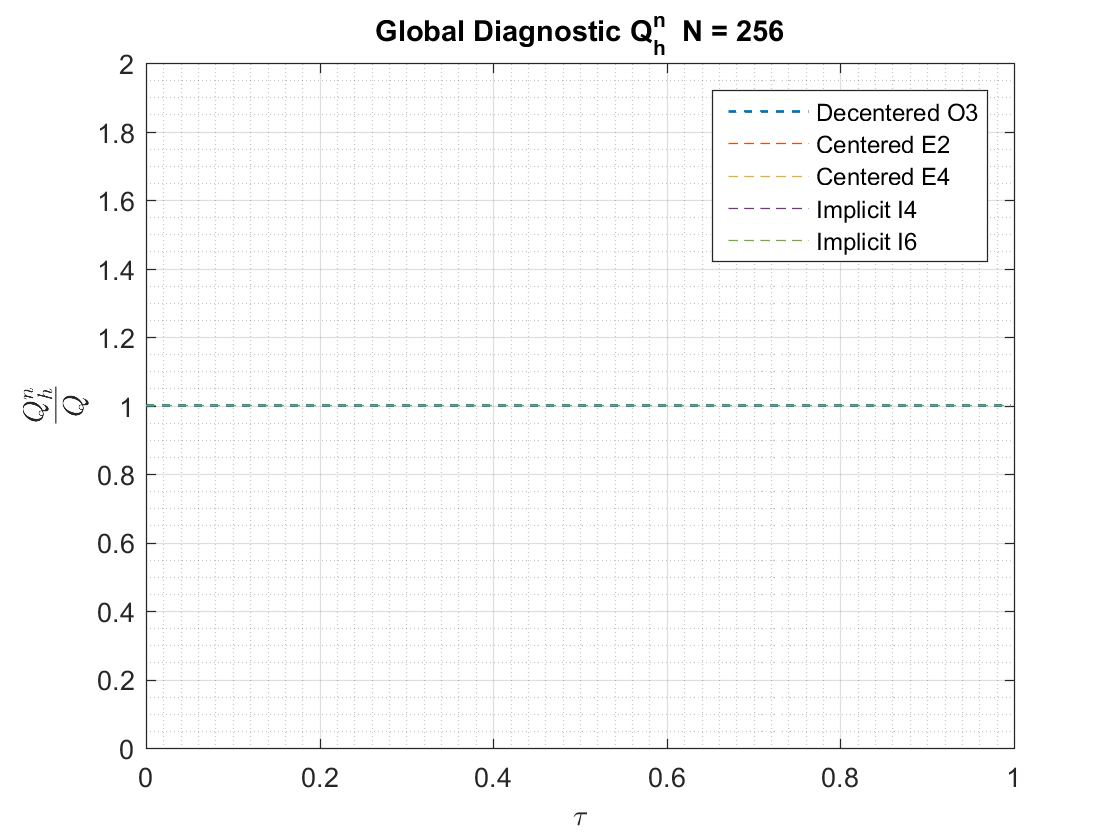
\includegraphics[scale=0.45]{img/fig6a.png}
    \caption{Diagnostique Globale $\frac{Q_h^n}{Q}$ N = 256 }
    \label{fig6a}
\end{figure}
\begin{figure}[H]
    \centering
    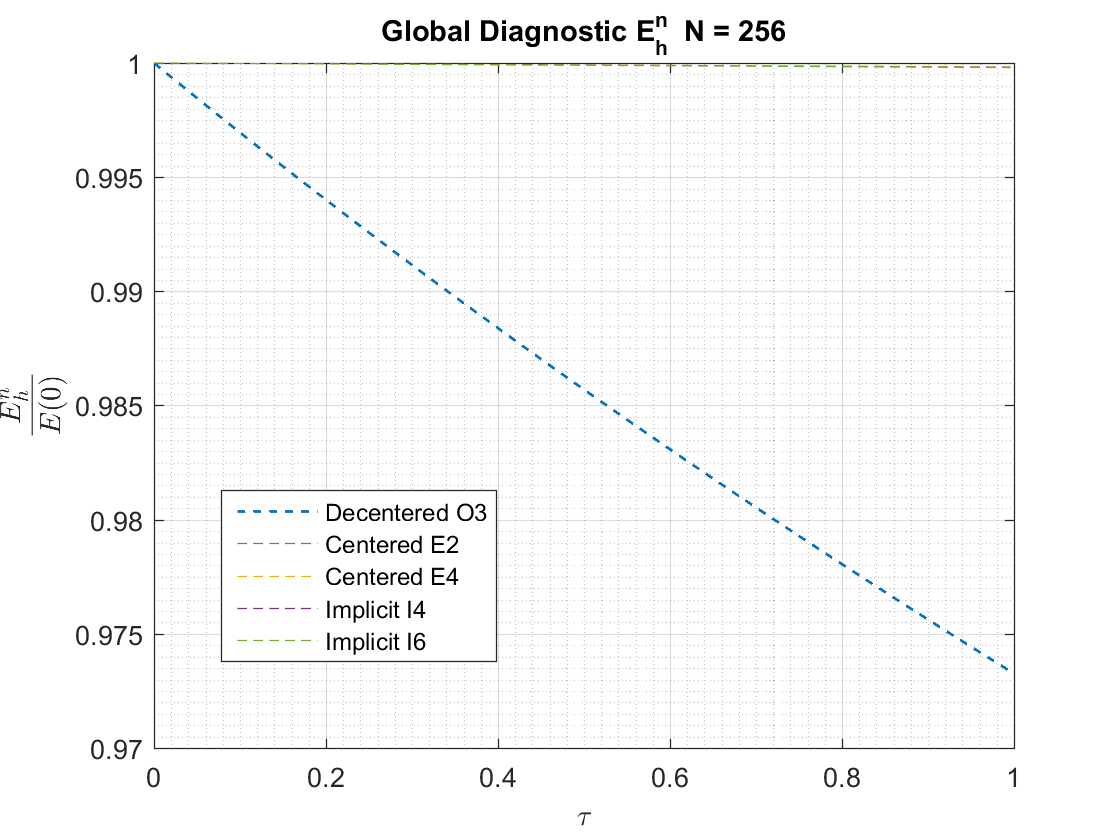
\includegraphics[scale=0.45]{img/fig6b.png}
    \caption{Diagnostique Globale $\frac{E_h^n}{E(0)}$ N = 256 }
    \label{fig6b}
\end{figure}
\begin{figure}[H]
    \centering
    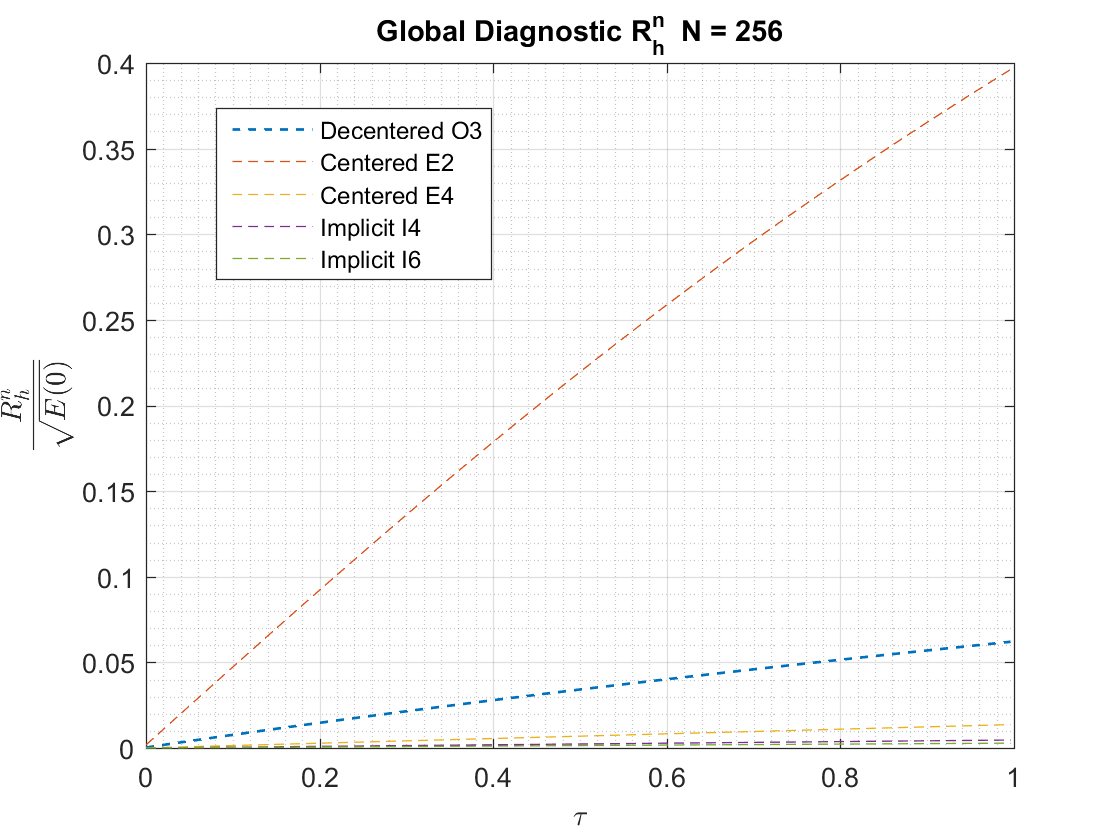
\includegraphics[scale=0.45]{img/fig6c.png}
    \caption{Diagnostique Globale $\frac{R_h^n}{\sqrt{E(0)}}$ N = 256 }
    \label{fig6c}
\end{figure}
\begin{figure}[H]
    \centering
    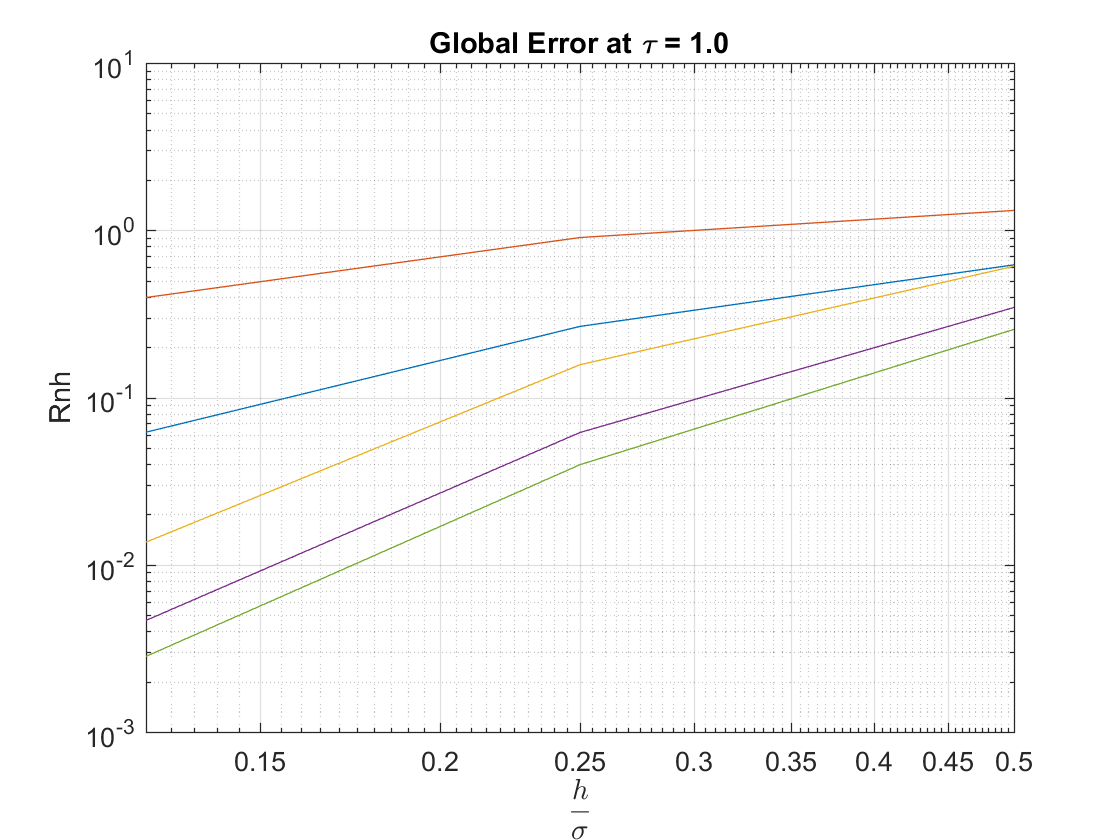
\includegraphics[scale=0.45]{img/fig9.png}
    \caption{Évolution de l'erreur global à $\tau = 1.0$ en fonction de $\frac{h}{sigma}$}
    \label{fig9}
\end{figure}
\newpage
\section{Simulation de la convection et de la diffusion}
Pour cette partie, on prendra à la place un $\frac{h}{\sigma}$ = 1/4, c'est à dire N = 128, avec un $Re_\sigma$ = 40. Nous utiliserons aussi une E2 pour déterminer notre dérivée seconde exprimé de la manière suivante:\\
\begin{equation}
    \frac{\partial^2 u}{\partial x^2} = \frac{ U_{i+1}-2U_i+U_{i-1} }{h^2} \\
\end{equation}
Puisque nous utilisons une différence finie d'ordre 2 pour la dérivée seconde, on se limitera au schéma de convection de E2, E4 et décentrée. Dès lors nous retrouvons les représentations suivantes, sur les figures \ref{fig5a}, \ref{fig5b}, \ref{fig5c}, et \ref{fig5d}. Contrairement à la convection pure, la décentré d'ordre 3 accouplé avec la E2 de diffusion semble moins dégénérer, si bien qu'elle suit relativement bien la solution exacte, certes pas aussi bien que la E4 de convection. Toutefois la E2 de convection s'éloigne toujours d'un peu la solution exacte. De plus, on remarque aussi que les instabilités de la E2 de convection s'atténue grâce à la diffusion. C'est un comportement qui se confirme avec les diagnostique globale des figures \ref{fig7a}, \ref{fig7b}, et \ref{fig7c}. En effet, alors que $Q_h^n$ reste bien constant, $E_h^n$ décrois quadratiquement pour les trois schémas, ce qui est due à la diffusion, et enfin nous apercevons bien que $R_h^n$ se stagne sur une sorte de plateau pour les 3 schémas, comme si il y avait une sorte d'amortissement pour l'erreur. Nous remarquons aussi que les valeurs sont aussi plus petites, mais nous investirons cela dans un autre point.
\begin{figure}[H]
    \centering
    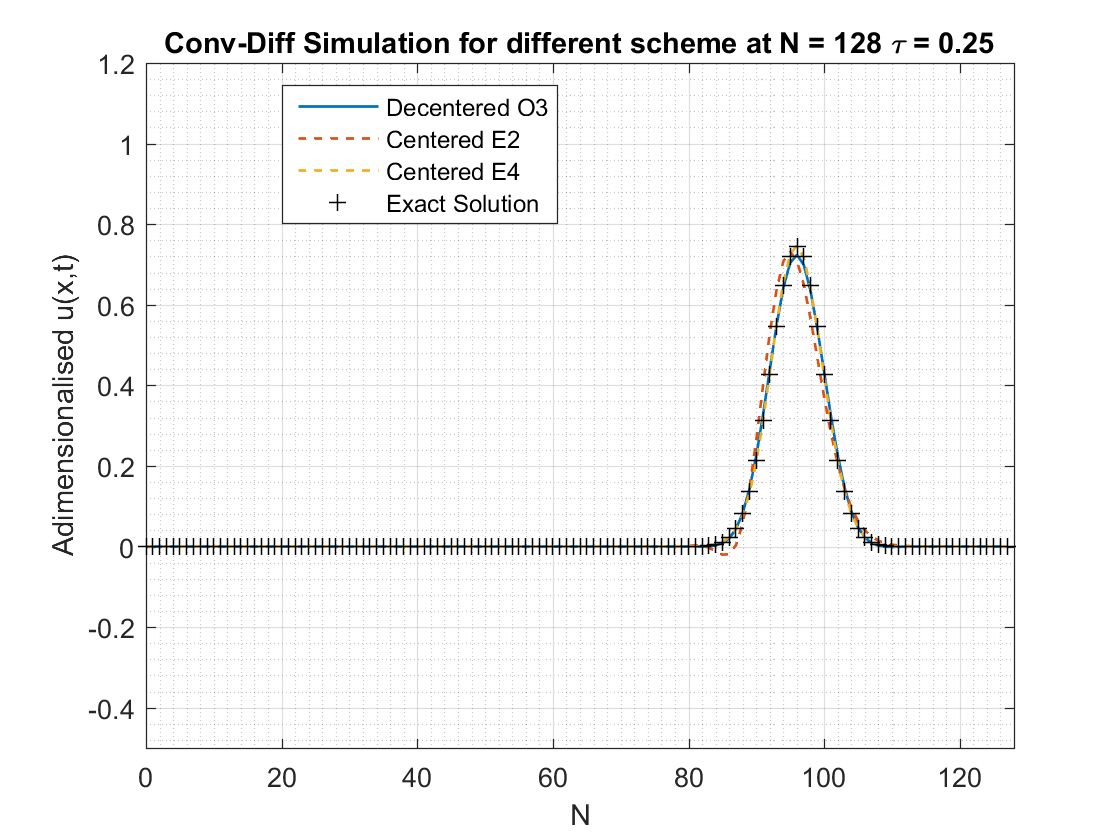
\includegraphics[scale=0.45]{img/fig5a.png}
    \caption{Réprésentation de $\frac{\sqrt{\pi \sigma^2}}{Q} U$ à $\tau$ = 0.25}
    \label{fig5a}
\end{figure}
\begin{figure}[H]
    \centering
    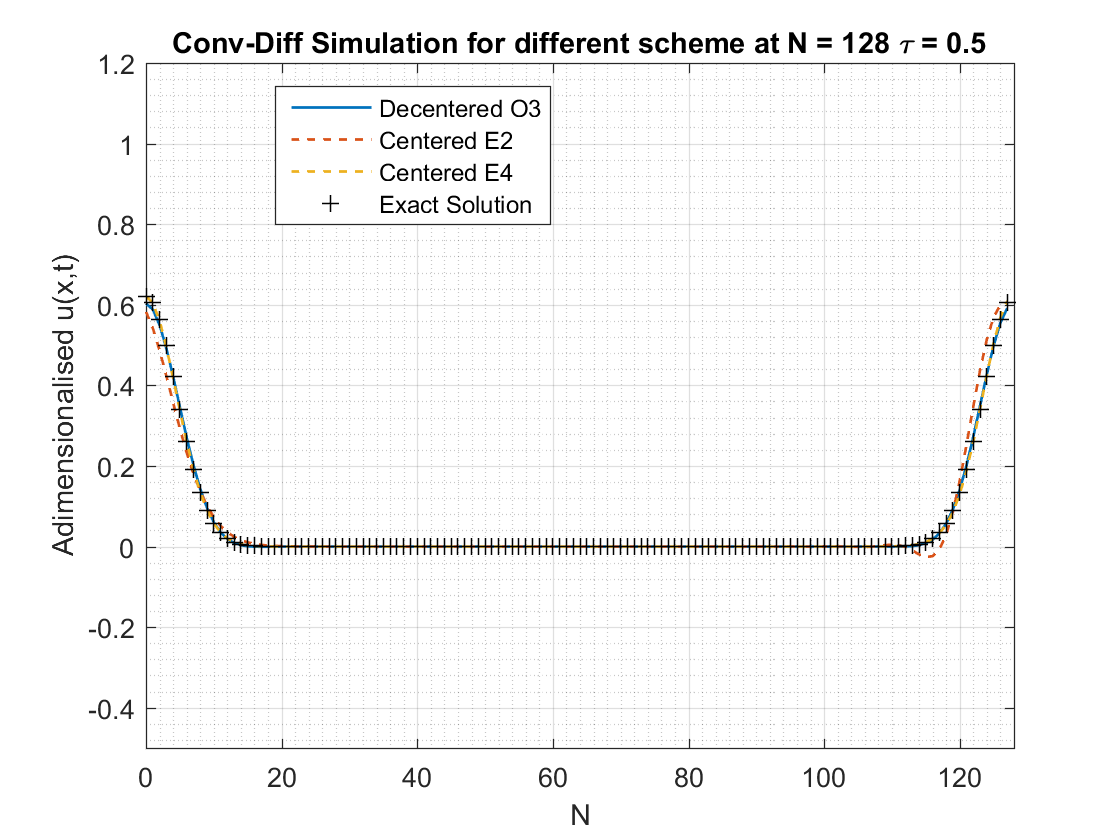
\includegraphics[scale=0.45]{img/fig5b.png}
    \caption{Réprésentation de $\frac{\sqrt{\pi \sigma^2}}{Q} U$ à $\tau$ = 0.50}
    \label{fig5b}
\end{figure}
\begin{figure}[H]
    \centering
    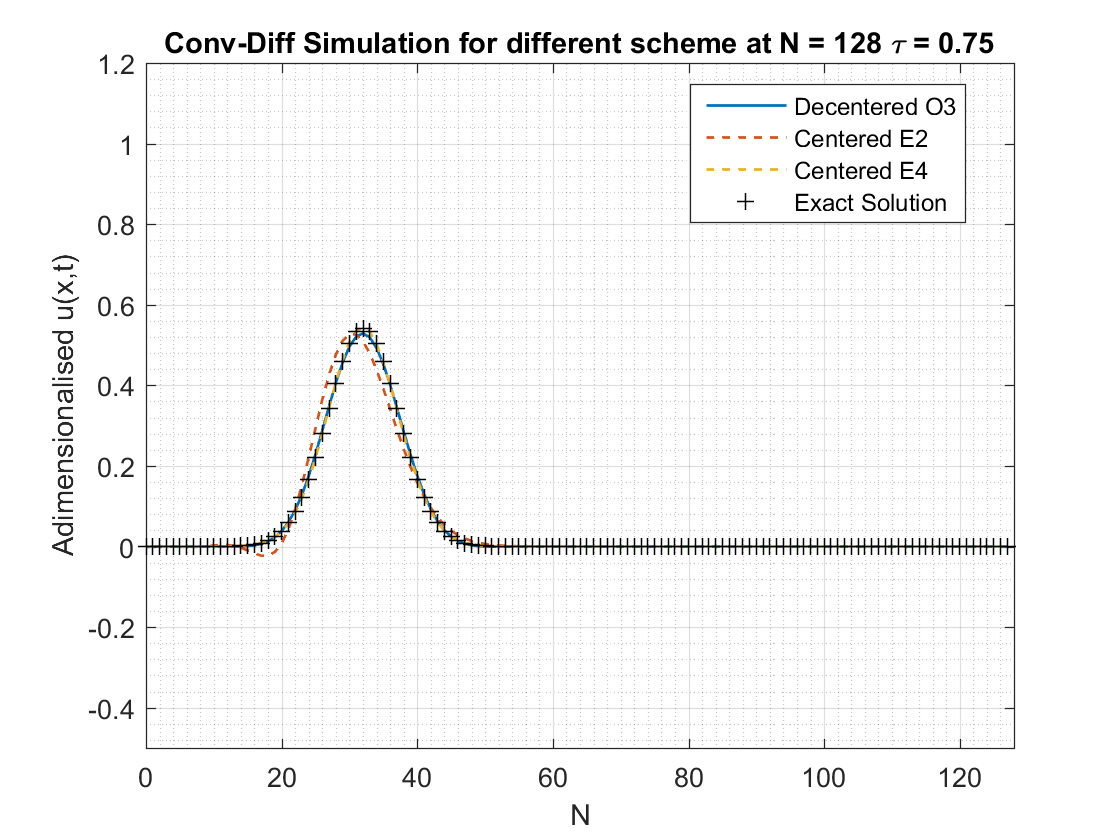
\includegraphics[scale=0.45]{img/fig5c.png}
    \caption{Réprésentation de $\frac{\sqrt{\pi \sigma^2}}{Q} U$ à $\tau$ = 0.75}
    \label{fig5c}
\end{figure}
\begin{figure}[H]
    \centering
    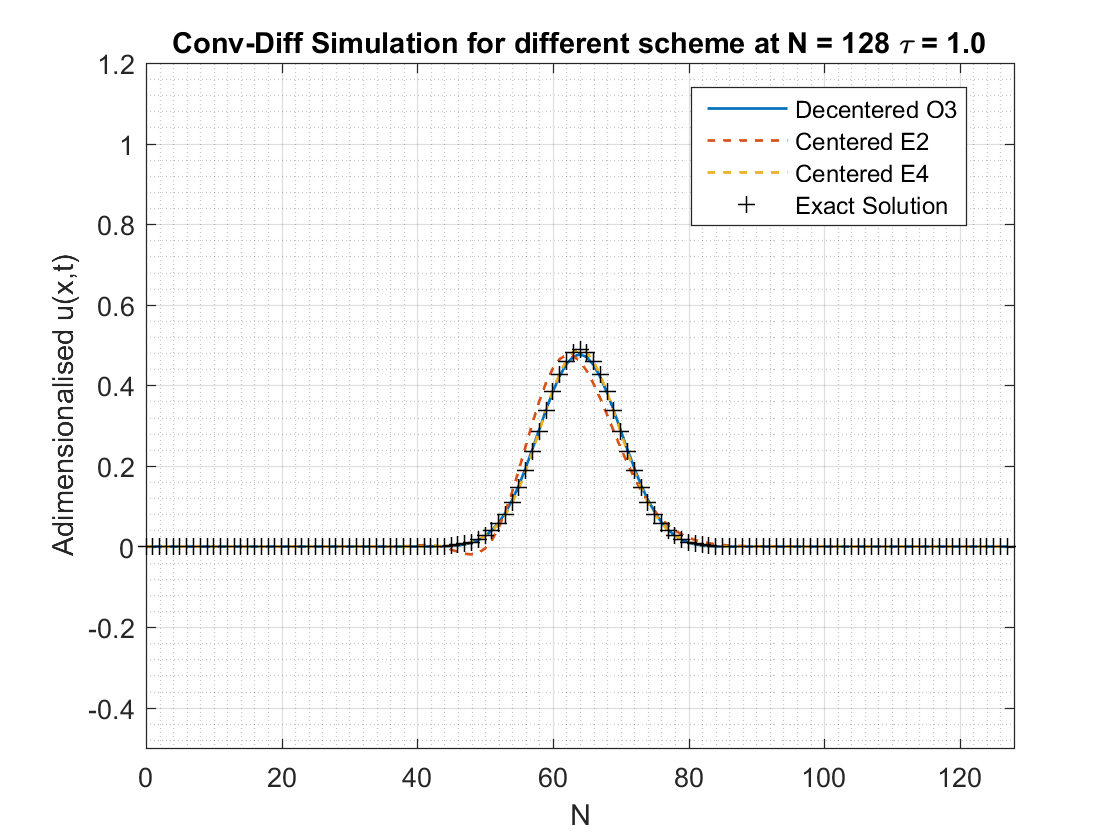
\includegraphics[scale=0.45]{img/fig5d.png}
    \caption{Réprésentation de $\frac{\sqrt{\pi \sigma^2}}{Q} U$ à $\tau$ = 1.00}
    \label{fig5d}
\end{figure}
\begin{figure}[H]
    \centering
    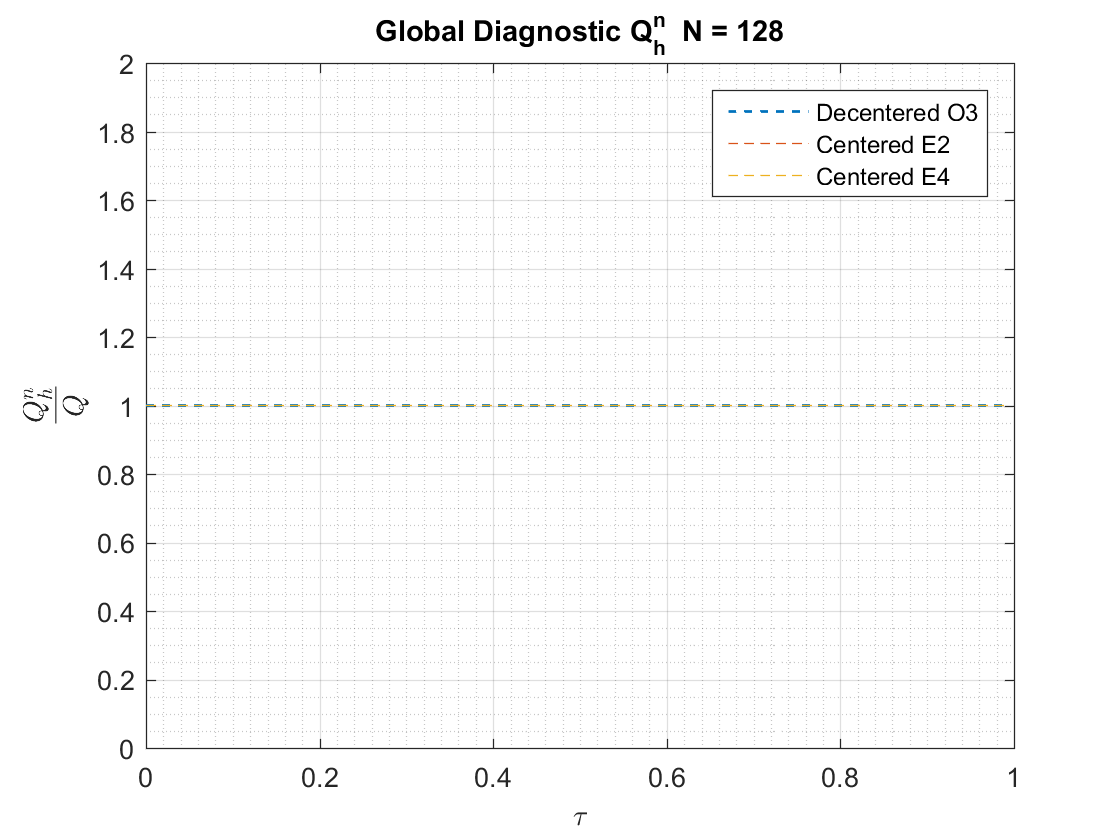
\includegraphics[scale=0.45]{img/fig7a.png}
    \caption{Diagnostique Globale $\frac{Q_h^n}{Q}$ N = 128}
    \label{fig7a}
\end{figure}
\begin{figure}[H]
    \centering
    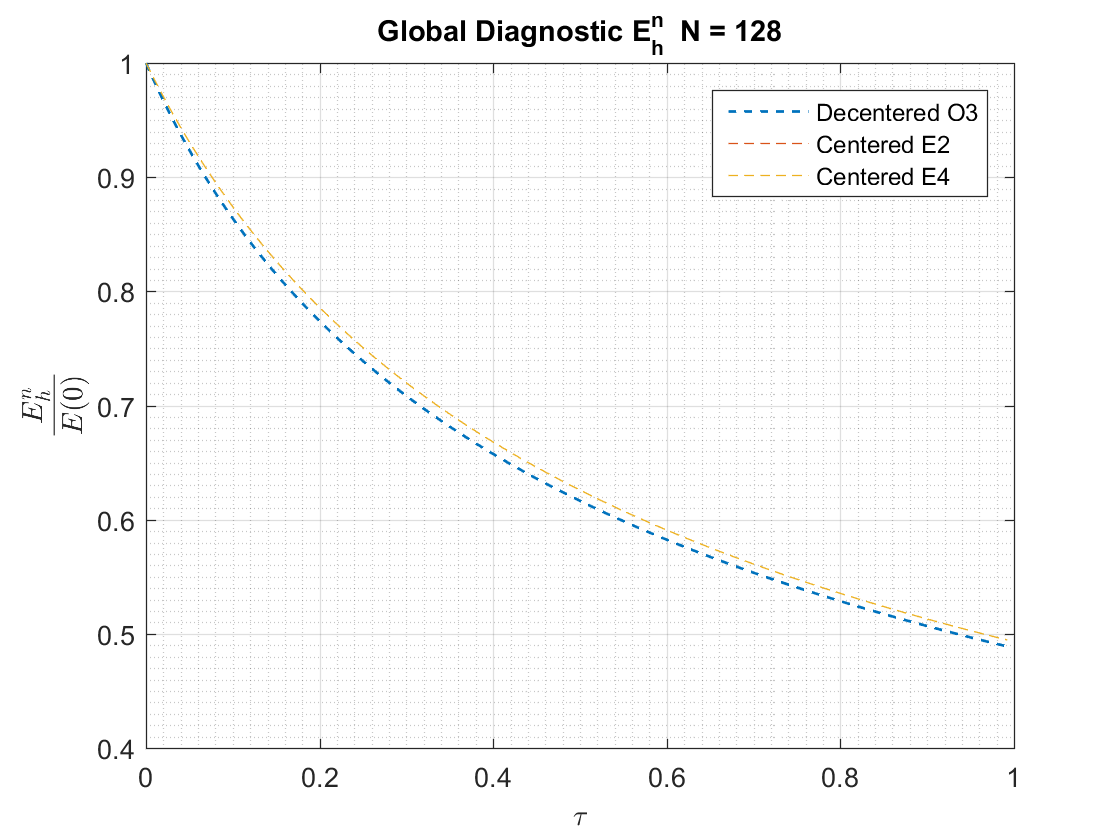
\includegraphics[scale=0.45]{img/fig7b.png}
    \caption{Diagnostique Globale $\frac{E_h^n}{Q}$ N = 128}
    \label{fig7b}
\end{figure}
\begin{figure}[H]
    \centering
    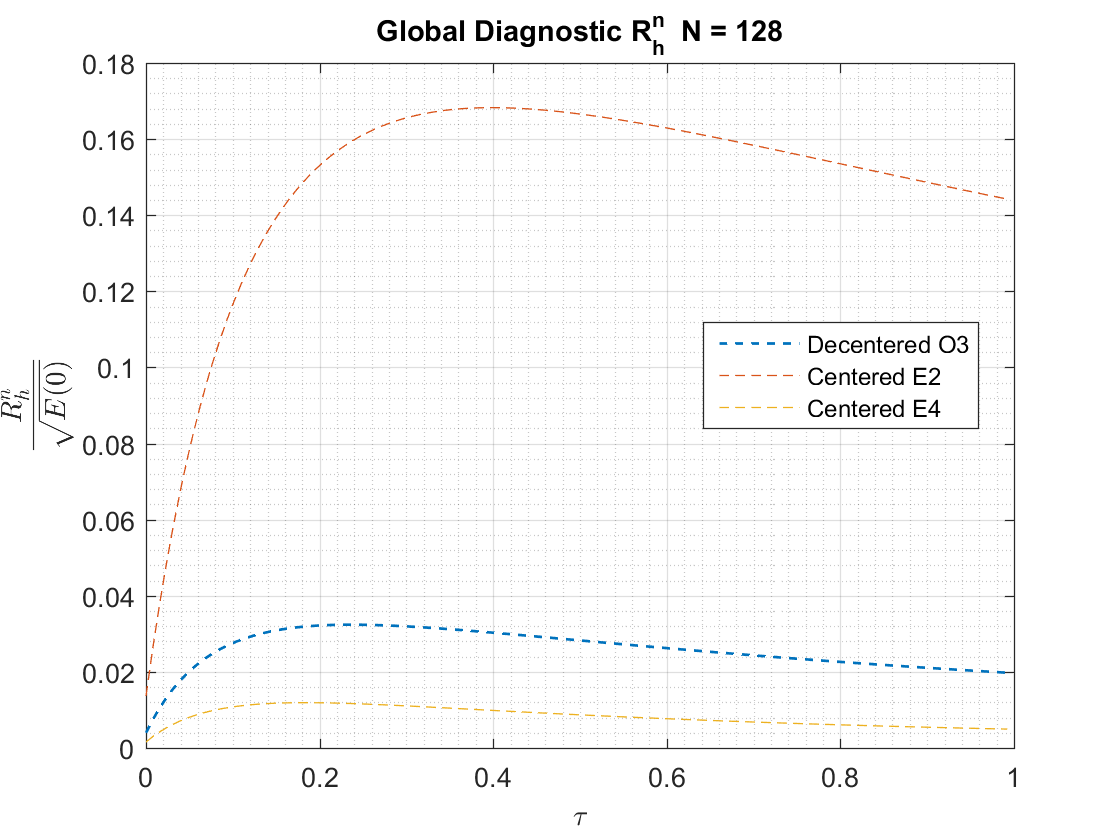
\includegraphics[scale=0.45]{img/fig7c.png}
    \caption{Diagnostique Globale $\frac{R_h^n}{Q}$ N = 128}
    \label{fig7c}
\end{figure}

\newpage
\section{Comparison Pure Convection vs Convection \& Diffusion}
Nous allons maintenant comparer notre convection-diffusion avec une convection pure, de ce fait nous allons utilisé dans les deux cas la décentrée d'ordre 3 pour le terme convectif, au temps $\tau = 0.75$ avec comme N = 128 ( $\frac{h}{\sigma} = \frac{1}{4}$). D'un premier coup d'oeil, on s'aperçoit, sur la figure \ref{fig8a},que la Conv-Diff possède une bien plutôt petite amplitude, de même qu'elle est un peu plus élargie que son voisin purement convectif. En obersvant les graphes de diagnostique, nous avons toujours un $Q_h^n$ constant, toutefois nous remarquons aussi que la pure convection semble diminuer plus rapidement en $E_h^n$ que la convection-diffusion. De même que nous voyons que l'erreur globale de la convection-diffusion s'atténue  bel et bien, et possède une plus petites valeurs que son voisin, comme on le remarquait précédemment, si bien qu'il a même l'impression de se corriger.
\begin{figure}[H]
    \centering
    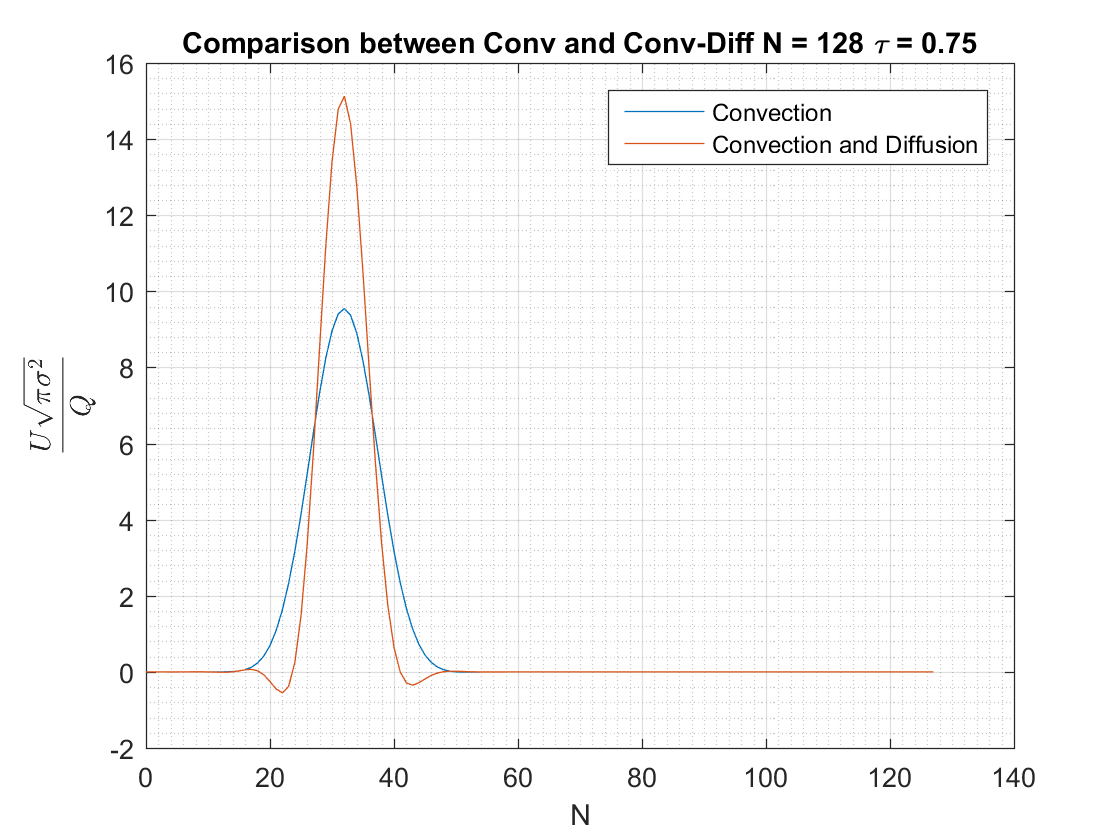
\includegraphics[scale=0.45]{img/fig8a.png}
    \caption{Réprésentation de $\frac{\sqrt{\pi \sigma^2}}{Q} U$  Pure-Conv vs Conv-Diff à $\tau$ = 0.75 N = 128}
    \label{fig8a}
\end{figure}
\begin{figure}[H]
    \centering
    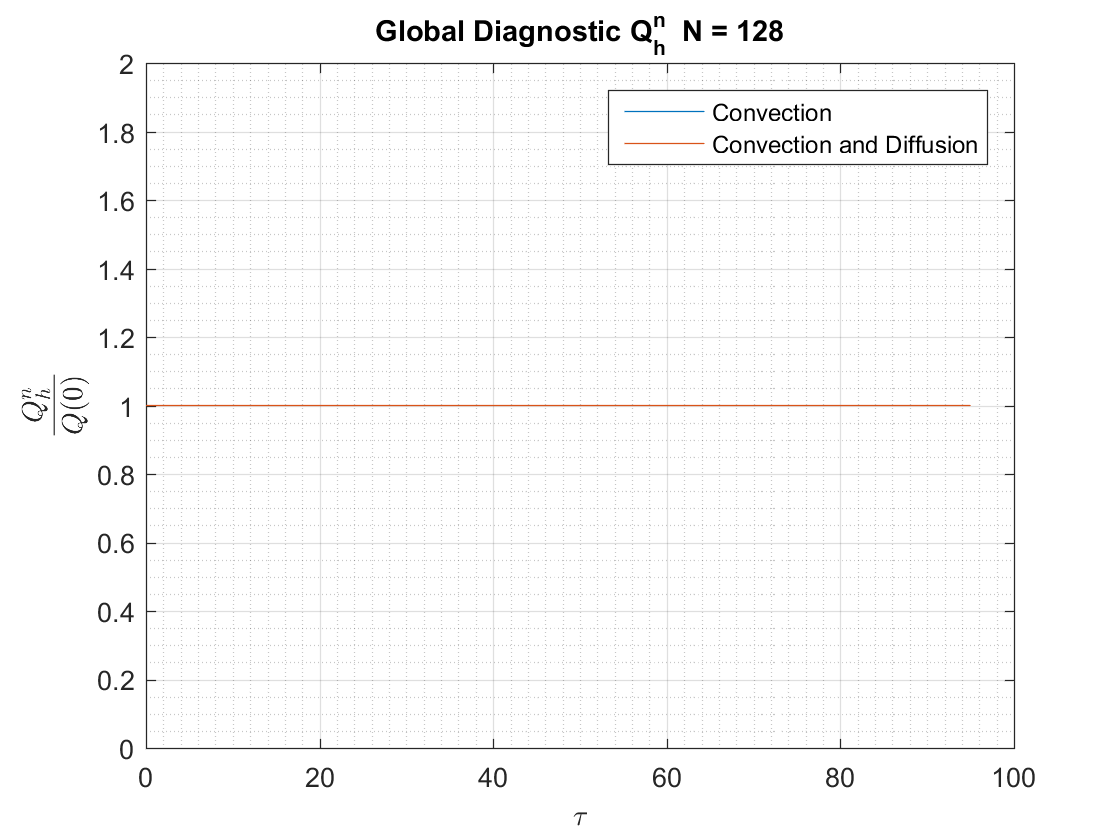
\includegraphics[scale=0.45]{img/fig8b.png}
    \caption{Diagnostique Globale $\frac{Q_h^n}{Q}$ Pure-Conv vs Conv-Diff N = 128}
    \label{fig8c}
\end{figure}
\begin{figure}[H]
    \centering
    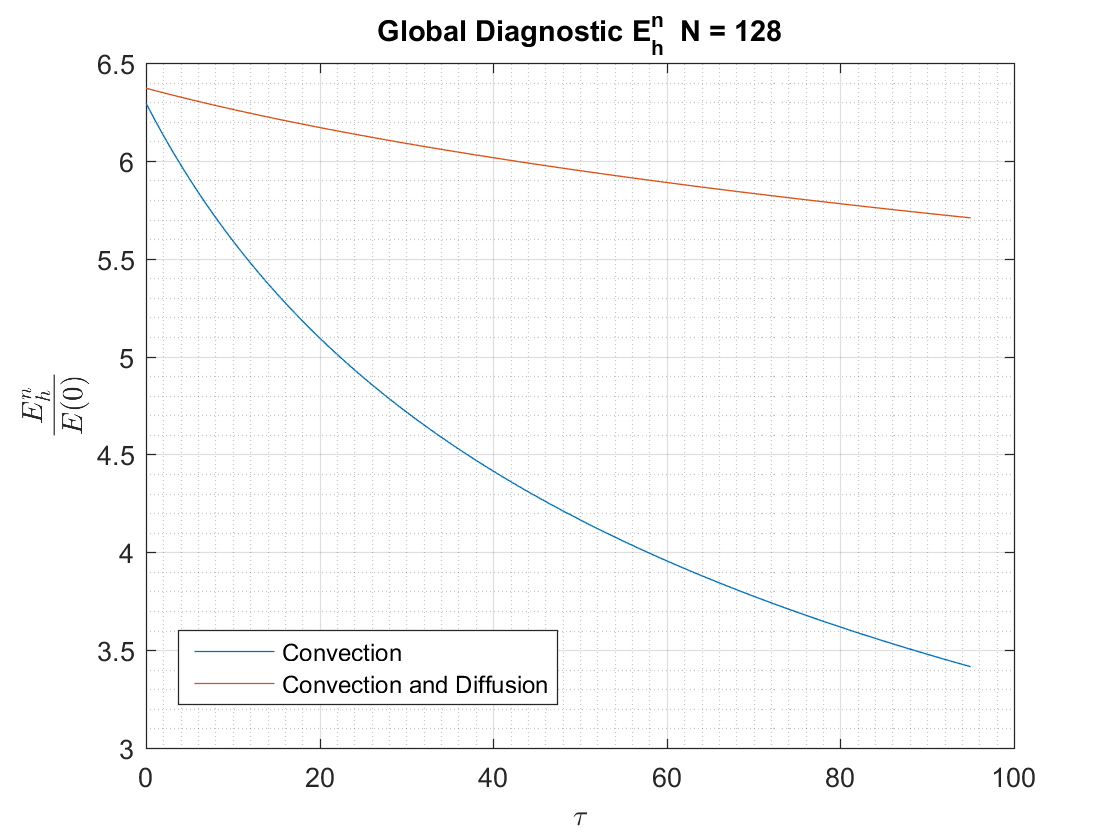
\includegraphics[scale=0.45]{img/fig8c.png}
    \caption{Diagnostique Globale $\frac{E_h^n}{Q}$ Pure-Conv vs Conv-Diff N = 128}
    \label{fig8c}
\end{figure}
\begin{figure}[H]
    \centering
    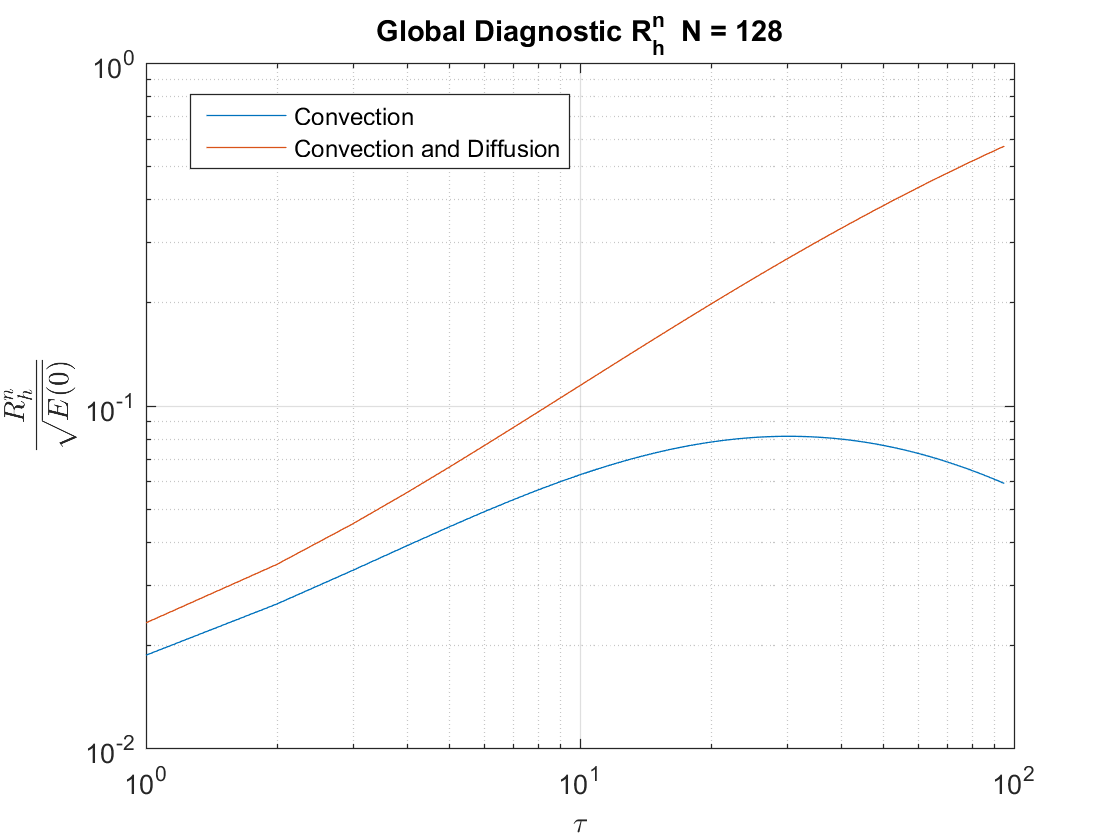
\includegraphics[scale=0.45]{img/fig8d.png}
    \caption{Diagnostique Globale $\frac{R_h^n}{Q}$ Pure-Conv vs Conv-Diff N = 128}
    \label{fig8d}
\end{figure}
\section{Bibliographie}
Un grand merci à tous ceux avec qui j'ai pu discuter et comparer mes résultats:\\
Julien Demey \\
Maxime Lejeune \\
Mathieu ????\\
Jérémie Waltzing \\

\end{document}
